\documentclass[a4paper,12pt,oneside]{memoir}

%documentation search
%http://texdoc.net/

%matematički paketi

\usepackage[intlimits]{amsmath}     %omogućava postavljanje granica integrala u formulama
\usepackage{amsthm}         %matematički teoremi, leme i sl.
\usepackage{siunitx}        %podrška za korištenje SI sustava mjernih jedinica
\usepackage{mathrsfs}
\usepackage{venndiagram}
\usepackage{nicefrac}

%encoding fontova i jezika
\usepackage[croatian]{babel}
\usepackage[utf8x]{inputenc}        %encoding inputa
\usepackage[enc=utf8]{hrlatex}
\usepackage[T1]{fontenc}        %encoding fontova koji je prikazan u PDF-u
\usepackage{amsfonts}
\usepackage{dsfont}

\usepackage[fixlanguage]{babelbib}
\selectbiblanguage{croatian}
\OnehalfSpacing

%\usepackage[datetime2-croatian]{datetime2}

%paketi tablica, naslova, poglavlja i sl.
\usepackage[thinlines]{easytable}
\usepackage{tocloft}        %upravljanje izgledom tablice sadržaja
\usepackage{pdfpages}       %integracija eksternih PDF-ova
\usepackage{booktabs}       %koristi se za formatiranje tablica sukladno standardu za znanstvene radove i članke
\usepackage{indentfirst}     %dodaje tab za svaku prvu rečenicu odlomka
\usepackage{subcaption}     %koristi se za podnaslove slika, formi i sl.
\usepackage[font=it]{caption}
\captionsetup[table]{position=above}
\captionsetup[figure]{position=below}
\captionsetup{labelsep=period}
\captionsetup{justification=centering}

\usepackage[hidelinks]{hyperref}        %podrška za integraciju hyperlinkova
\urlstyle{same}

\usepackage{float}
%grafički paketi
% \usepackage{pgfcore}
% \usepgflibrary{datavisualization.formats.functions}
\usepackage{graphicx}
\usepackage{multirow}
\usepackage{pgfmath}
\usepackage{pgfplots}
\usepgfplotslibrary{statistics}
\usepackage{pgfplotstable}
\pgfplotsset{compat=1.17}
\pgfplotsset{
    standard/.style={
        width = 0.9\linewidth,
        semithick,
        tick style={major tick length=4pt,semithick,black},
        every axis plot post/.style={mark options={fill=black}},
        separate axis lines,
        axis x line*=bottom,
        axis x line shift=5pt,
        %xlabel shift=5pt,
        axis y line*=left,
        axis y line shift=5pt,
        ylabel shift=5pt,
        xtick align = outside,
        ytick align = outside,
        xlabel near ticks,
        ylabel near ticks,
        % xmin = -2, xmax = 2,
        % ymin = -1, ymax = 1,
        grid = both
    }
}
\usepackage{tikz}
\usetikzlibrary{datavisualization}
\usetikzlibrary{datavisualization.formats.functions}
\usetikzlibrary{arrows,automata,patterns,positioning,shapes}
\tikzstyle{block}=[draw, fill=gray!20, rectangle, minimum size=1.5em]
\tikzstyle{sum} = [draw, fill=gray!20, circle, node distance=4cm, minimum size=2em]
% \tikzset{
%     sum/.style n arg = {4}[draw, circle, node distance = 2cm, minimum size=5mm, alias=sum, append after command={
%     node at (sum.north) [port, below=1pt] {$#1$}
%     node at (sum.west) [port, right=1pt] {$#2$}
%     node at (sum.south) [port, above=1pt] {$#3$}
%     node at (sum.east) [port, left=1pt] {$#4$}
% }]}
\tikzstyle{input} = [coordinate]
\tikzstyle{output} = [coordinate]
\tikzstyle{pinstyle} = [pin edge={to-,thin,black}]
\tikzstyle{init} = [pin edge={to-,thin,black}]
\usepackage{circuitikz}
\newcommand{\pgfmathparseFPU}[1]{\begingroup%
\pgfkeys{/pgf/fpu,/pgf/fpu/output format=fixed}%
\pgfmathparse{#1}%
\pgfmathsmuggle\pgfmathresult\endgroup}
\pgfmathdeclarefunction{gauss}{2}{%
  \pgfmathparse{1/(#2*sqrt(2*pi))*exp(-((x-#1)^2)/(2*#2^2))}%
}


%misc. paketi

\usepackage{soul} %žuti marker
\usepackage{times}

%formatiranje dokumenta
\pagestyle{myheadings}
\setulmarginsandblock{2.5cm}{2.5cm}{*}
\setlrmarginsandblock{2.5cm}{2cm}{*}
\checkandfixthelayout

\setlength{\parskip}{6pt} %razmak između odlomaka

\usepackage{titlesec}   %nadomješta LaTeX makroe za naslove, odlonke, itd.

\titleformat{\chapter}
{\normalfont\fontsize{14}{14}\bfseries}
{\thechapter}
{1em}
{}
\titlespacing{\chapter}{0pt}{*4}{*1}
\titleformat{\section}
{\normalfont\fontsize{12}{14}\bfseries}
{\thesection}
{1em}
{}
\titlespacing{\section}{0pt}{*4}{*1}
\setsecnumdepth{subsection}
\maxtocdepth{subsection}
\titleformat{\subsection}
{\normalfont\fontsize{12}{14}}
{\thesubsection}
{1em}
{}
\titlespacing{\subsection}{0pt}{*4}{*1}

%formatiranje dokumenta - dodavanje točaka u naslove

\renewcommand{\thechapter}{\arabic{chapter}.}
\renewcommand{\thesection}{\thechapter\arabic{section}.}
\renewcommand{\thesubsection}{\thesection\arabic{subsection}.}

%formatiranje dokumenta - promjena fonta naslova "Sadržaj"

\renewcommand\printtoctitle[1]{\normalfont\fontsize{14}{14}\bfseries #1}

%formatiranje dokumenta - promjena riječi "Dodatak" u sadržaju

\renewcommand*{\cftappendixname}{Dodatak\space}

%formatiranje dokumenta - numeriranja tablica i slika



\renewcommand{\thetable}{\thechapter\arabic{table}}
\renewcommand{\thefigure}{\thechapter\arabic{figure}}

%teoremi

\newtheorem{theorem}{Teorem}[chapter]
\newtheorem{korolar}{Korolar}[chapter]
\newtheorem{definition}{Definicija}[chapter]
\newtheorem{lema}{Lema}[chapter]
\newtheorem{prop}{Propozicija}[chapter]
\newtheorem{primjer}{Primjer}[chapter]

%formule

\newcommand{\fourierovred}{f(x)= \frac{a_0}{2}+\sum_{n=1}^\infty (a_n cos(nx)+b_n sin(nx))}
\newcommand{\nasavjerojatnost}{p(t)= \frac{e^{a+b\cdot t}}{1+e^{a+b\cdot t}}}
\newcommand{\kauzalni}{y[n]=\frac{1}{M}\displaystyle\sum_{k=0}^{M-1 }x[n-k]}
\newcommand{\nekauzalni}{y[n]=\displaystyle\sum_{k=-\infty}^{n}x[n-k]}

%primjer parametriziranih TikZ grafova
%http://www.texample.net/tikz/examples/parameterized-plots/

%primjer normalne razdiobe
%http://www.texample.net/tikz/examples/tikzdevice-demo/

%formatiranje dokumenta - numeriranja jednadžbi, definicija i teorema

\renewcommand\theequation{\thechapter\arabic{equation}}
\renewcommand\thetheorem{\thechapter\arabic{theorem}}
\renewcommand\thedefinition{\thechapter\arabic{definition}}
\renewcommand\thekorolar{\thechapter\arabic{korolar}}
\renewcommand\theprimjer{\thechapter\arabic{primjer}}


\author{Denis Mijolović} 

\begin{document}
    \begin{titlingpage}
        \begin{center}\linespread{1.8}\fontsize{16}{16}
            \normalfont{
                SVEUČILIŠTE U RIJECI
            }\\
            {\textbf{
                TEHNIČKI FAKULTET
                }
            }\\
        \fontsize{14}{14}\normalfont{
            Preddiplomski sveučilišni studij elektrotehnike
        }            
        \end{center}
        \vspace{6cm}
        \begin{center}\linespread{1.8}
            \fontsize{14}{14}\normalfont{
                Završni rad
            }\\
            \fontsize{16}{16}{\textbf{
                AUTOREGRESIJSKI MODELI U OBRADI SIGNALA
                }
            }
        \end{center}
        \vspace{6cm}
        \vfill\noindent
        \begin{tabular}[t]{l@{}}
            \fontsize{14}{14}\normalfont{
                Rijeka, \today
            }
        \end{tabular}
        \hfill
        \begin{tabular}[t]{l@{}}
            \fontsize{14}{14}\normalfont{
                Denis Mijolović
            }\\
            \fontsize{14}{14}\normalfont{
                0069066432
            }
        \end{tabular}
        \thispagestyle{empty}
        \newpage
            \begin{center}\linespread{1.8}
                \fontsize{16}{16}\normalfont{
                    SVEUČILIŠTE U RIJECI
                }\\
                {\textbf{
                    TEHNIČKI FAKULTET
                    }
                }\\
                \fontsize{14}{14}\normalfont{
                    Preddiplomski sveučilišni studij elektrotehnike
                }
            \end{center}
            \vspace{6cm}
            \begin{center}\linespread{1.8}
                \fontsize{14}{14}\normalfont{
                    Završni rad
                }\\
                \fontsize{16}{16}{\textbf{
                    AUTOREGRESIJSKI MODELI U OBRADI SIGNALA
                    }
                }\\
                \fontsize{14}{14}\normalfont{
                Mentor: doc. dr. sc. Ivan Dražić
            }\\
            \fontsize{14}{14}\normalfont{
                Komentor: prof. dr. sc. Viktor Sučić
            }
            \end{center}
        \vfill\noindent
        \begin{tabular}[t]{@{}l}
            \fontsize{14}{14}\normalfont{
                Rijeka, \today
            }        
        \end{tabular}
        \hfill
        \begin{tabular}[t]{@{}l}
            \fontsize{14}{14}\normalfont{
                Denis Mijolović
            }\\
            \fontsize{14}{14}\normalfont{
                0069066432
            }
        \end{tabular}
        \thispagestyle{empty}
        \newpage
            \thispagestyle{empty}
            
\includepdf{zavrsni_rad_zadatak.pdf}
        \newpage
            \thispagestyle{empty}
            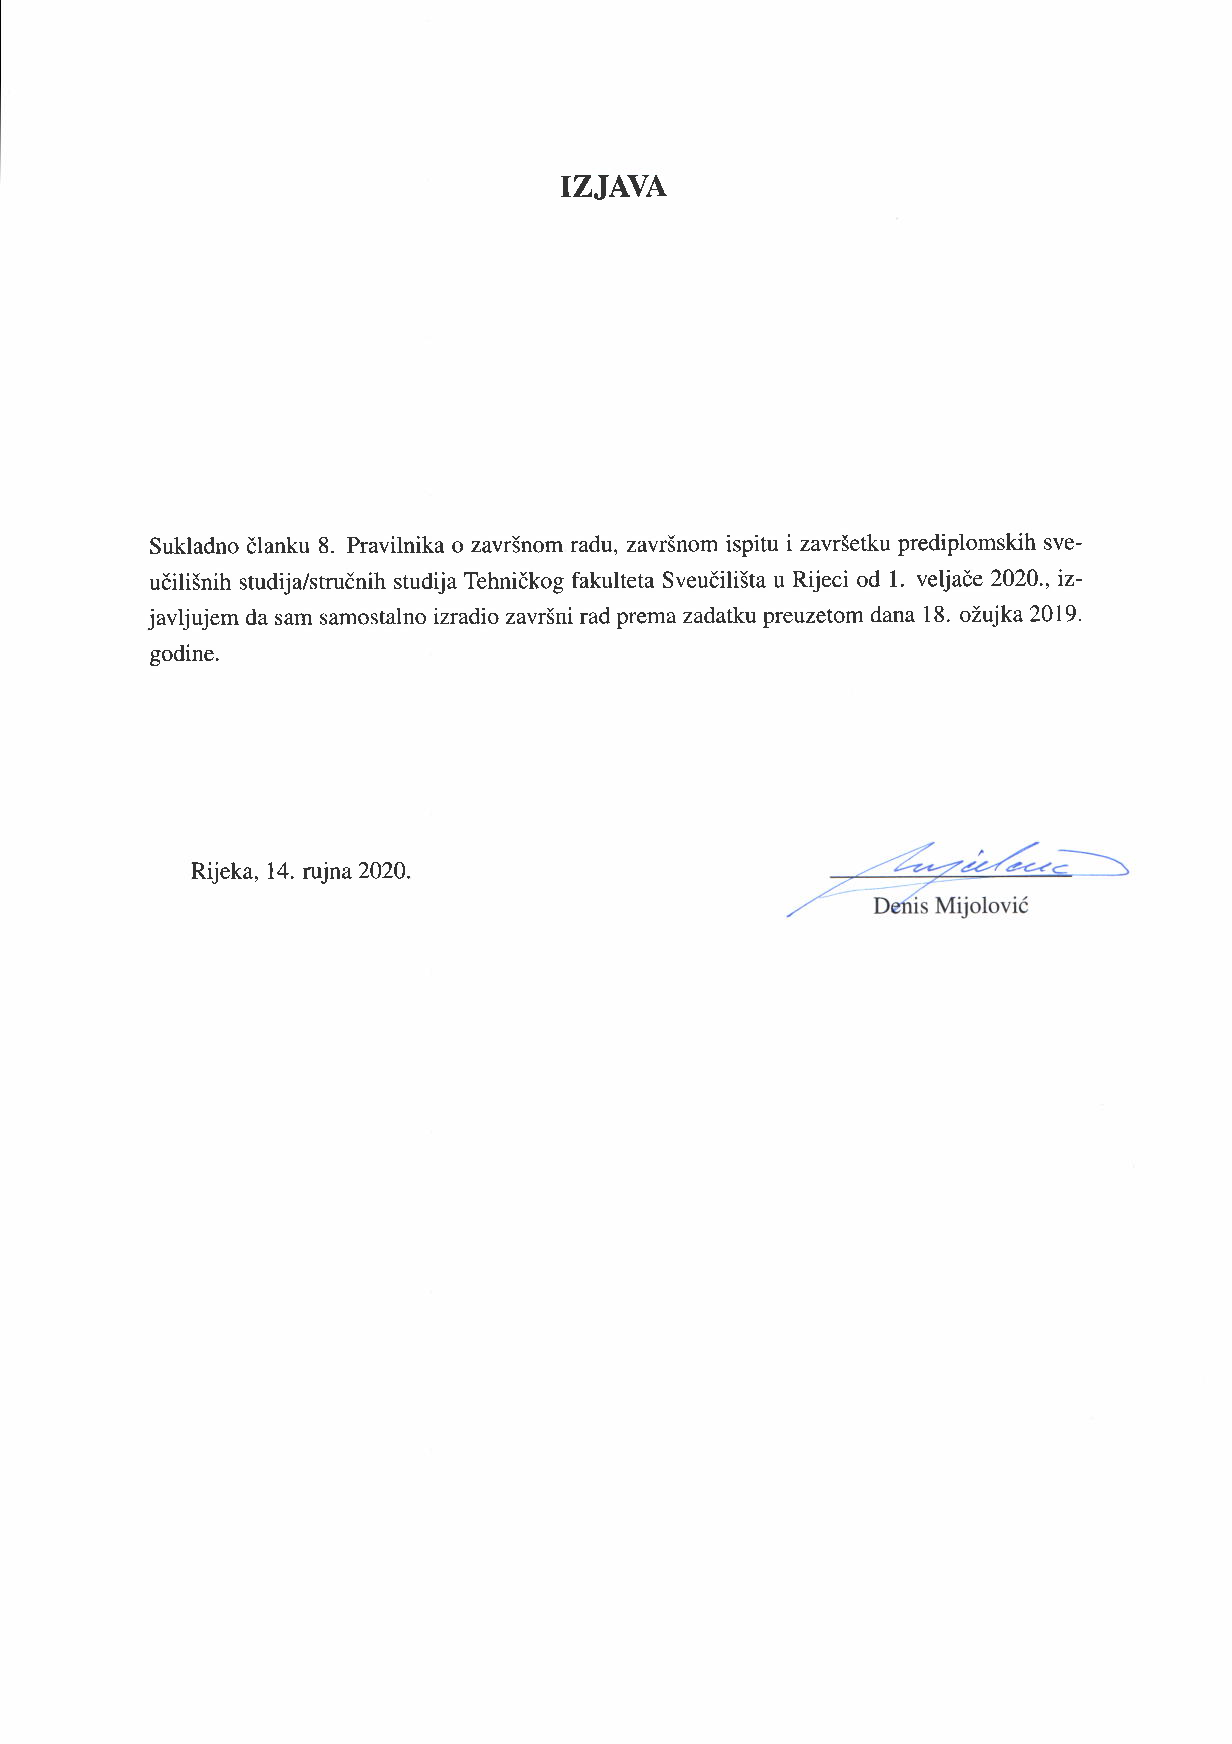
\includepdf{izjava_autenticnost.pdf}
            %     \begin{center}\linespread{1.8}\fontsize{16}{16}
            %         {\textbf{
            %             IZJAVA
            %             }
            %         }
            %     \end{center}
            % \vspace{5cm}
            % Sukladno članku 8. Pravilnika o završnom radu, završnom ispitu i završetku prediplomskih sveučilišnih studija/stručnih studija
			% Tehničkog fakulteta Sveučilišta u Rijeci od 1. veljače 2020., izjavljujem da sam samostalno izradio završni rad
            % prema zadatku preuzetom dana 18. ožujka 2019. godine.
            % \vspace{3cm}


            % \begin{tabular}[t]{@{}l}
            %     \normalfont{
            %         Rijeka, 14. rujna 2020.
            %     }
            % \end{tabular}
            % \hfill
            % \begin{tabular}[t]{@{}l} 
            %     \fontsize{14}{14}\hrulefill\\
            %     \fontsize{12}{12}\normalfont{
            %         \phantom{Raz}Denis Mijolović\phantom{Raz}
            %     }
            % \end{tabular}
            \newpage
                \thispagestyle{empty}
                $ $
                    \vspace{5cm}
                    \textit{
                        \\
                        Lorem ipsum dolor sit amet, consectetur adipiscing elit. Mauris et ante a mauris consequat tempor. Donec vulputate, nulla pharetra finibus finibus, ipsum ante molestie mauris, in tincidunt libero augue sit amet arcu. In hac habitasse platea dictumst. Nulla sagittis ante ac augue volutpat cursus. Ut gravida odio malesuada, vestibulum mi at, dignissim leo. Morbi semper finibus est, id maximus mauris auctor eget.
                    }
    \end{titlingpage}
    \begin{KeepFromToc}
        \tableofcontents
    \end{KeepFromToc}
    \chapter{Uvod}
        %Potrebno je prepraviti uvod na način da opisuje povod za pisanje završnog rada -- dodati malo elektrotehnike u priču
        \textbf{(Definicija podataka i informacija na zanimljiv način...ako je takvo što moguće)}

        Vratimo li se u prošlost, važnost podataka i njihova inerpretacija u svrhu stvaranja informacija bila je neminovna za civilizacijske strukture koje danas poznajemo. Od početka razvoja primitnivnih tehnologija i njezinoga korištenja za optimizaciju životnih procesa, do razvoja trgovine i financijskih instrumenata; čovjek je sve efikasnije koračao prema evolucijskom vrhu uspješnom utilizacijom svoje okoline. Daljnjim razvojem, čovjek je nadišao barijeru vlastite memorije za obradu podataka, te se počeo približavati točki zasićenja - uslijed koje se javila potreba za stvaranjem boljega i efikasnijega načina obrade podataka i njihove pretvorbe u sažetiju i jednako kvalitetnu informaciju.

        Kao i kod većine velikih znanstvenih otkrića koja su obilježila svoje razdoblje kao pretkretnice stoljeća u ratnim okolnostima, tako je i tijekom Drugog svjetskog rata otkriven novi izum kao odgovor na Enigmu - stroj koji je kodirao njemačke vojne i diplomatske poruke te čija se šifra smatrala nerješivom. Uzevši u obzir širenje nacističke Njemačke i prijetnju koja je prijetila ljudskim slobodama, javila se jasna potreba za stvaranjem rješenja koje će nadići čovjekova fizička i psihička ograničenja te biti u mogućnosti procesuirati veliku količinu podataka u vrlo kratkom vremenu -- radeći neprestano i ne osjećajući umor te, konzekventno, ne stvarajući greške. Imajući to na umu, Englezi su tada izumili \textit{Colossus} -- uređaj koji je pomogao kriptoanalitičarima da dešifriraju njemačke poruke i dao im stratešku prednost pri prognozorianju daljnih koraka tijekom ratnog razdoblja. Taj uređaj se u današnje vrijeme smatra pretečom prvoga računala kakvim ga danas poznajemo.

        Baš kao i tada, te kroz cijelu ljudsku povijest, ispravna interpretacija podataka u informaciju koju krajnji korisnik može iskoristiti u svrhu kvalitetnijeg donošenja važnih odluka, iskazala se kao značajan faktor u očuvanju civilizacijske i sveopće stabilnosti -- stanja koje je najpotentnije za budući razvoj, a time i blagostanje. Kako je civilizacija težila ka tehnološkom društvu, tako je eksponencijalno rasla i količina podataka koju je bilo potrebno interpretirati; te se javila potreba za sve preciznijim prognoziranjem budućega ponašanja sustava kako ne bi došlo do destrukcije vitalnih procesa i porasta volatilnosti sustava - a samim time i povećanjem vjerojatnosti za njegovim urušavanjem.

        Slijedno tome, važnost prognoziranja proizlazi iz dvije osnovne činjenice:
        \begin{enumerate}
            \item budućnost je nepredvidiva
            \item poduzete akcije u vrijeme donošenja odluke vrlo često nemaju trenutne posljedice sve do određenoga trenutka u budućnosti
        \end{enumerate}


        Imajući na umu prethodno navedene činjenice, slijedno je zaključiti da precizne prognoze budućih događaja pospješuju efikasnost postupka donošenja odluka. Štoviše, većina odluka od posebnog poslovnog ili političkog značaja imaju nužan uvjet pozitivnih prognostičkih indikatora prezentiranih kroz studije izvedivnosti ili ispitivanja javnoga mnijenja -- čija je zadaća što preciznije prognozirati buduću potražnju za proizvodima i uslugama koje su predmet proizvodnih, industrijskih ili inih procesa. U konkretnijem, mikroekonomskom smislu, dalo bi se konstatirati da je prognoziranje implementirano u gotovo sve odluke koje su dio naše svakodnevice: poduzeće će početi izgradnju nove proizvodne jedinice kako bi osiguralo rastuću potražnju na tržištu; zaposleni radnici početi će štedjeti kako bi si mogli priuštiti godišni odmor ili kupnju vrijednosnica s ciljem ostvarivanja prava na buduću kapitalnu dobit; rektor sveučilišta donesti će odluku o otvaranju novog studijskog programa kako bi povećao broj studenata i uskladio broj obrazovanih stručnjaka s budućim tržišnim potrebama. Ukratko, svaki od navedenih procesa zahtjeva inicijalnu percepciju utjecaja donešenih odluka na povećanje vjerojatnosti ostvarivanja zadanih ciljeva -- i to prije donošenja samih odluka.


        Ostanemo li na mikroekonomskoj razini, možemo reći da je poslovanje poduzeća zahvaćeno trima faktorima: makroekonomskim prilikama, industrijskim pokazateljima i samim uređenjem poduzeća. Obzirom da direktor takvoga poduzeća najčešće ima mogućnost direktnoga djelovanja jedino na poslijednja dva faktora, od iznimne je važnosti da bude što bolje informiran o vanjskim utjecajima i trendovima na koje ne može izravno djelovati -- poput donošenja novih zakonskih regulativa ili razvoja globalne virusne pandemije. Važnost ispravnog prognoziranja čimbenika na koje se nema direktan utjecaj od iznimne je važnosti za većinu projekta iznimno velike vrijednosti. Tako, na prijmer, projekti s velikim početnim ulaganjima poput izgradnje novih jedinica za opskrbu električnom energijom, mogu imati vrijeme izrade studije izvedivosti u trajanju od 10 ili više godina prije nego što li se započnu radovi. Budući da opskrba električnom energijom ovisi o stupnju razvijenosti regije ili područja, potrebno je izraditi valjane prognoze koje će pomoći u procjeni trenutne, kratkoročne i dugoročne isplativosti novih opskrbnih jedinica za opskrbljivača, ostale projektne partnere, te za lokalni i regijalni razvoj. U tom slučaju, prisutnost raznovrsnih rizika utječe na sve dionike projekta -- od nacionalne, regionalne ili lokalne uprave ili samouprave; do svih industrijskih poduzeća koja se nalaze na tom području. Ti rizici mogu biti smanjenje likvidnosti tržišta, kreditni status\footnote{Usporedba potraživanja i dugovanja nekoga poduzeća koje se dalje koriste za utvrđivanje kreditnog rejtinga.}, kamatni rizik\footnote{Moguće smanjenje vrijednosti financijskih instrumenata javno dostupnoga poduzeća uslijed promjene razine kamatnih stopa na tržištu.},valutni rizik\footnote{Osjetljivost financijskih instrumenata na fluktuacije tečajeva stranih valuta. Značajno za multinacionalna poduzeća s viševalutnim potraživanjima i dugovanjima.}, strateški rizik\footnote{Rizik za prihode ili kapital koji nastaje kao posljedica neadekvatnih poslovnih odluka ili nepravilnog vođenja poduzeća.}, stanje tržišta rada i još mnogi drugi. Pritom je važno napomenti važnost osjetljivosti modela prognoziranja na fluktuacije u svakoj stavci procjene ukupnoga rizika, tj. isti prognostički model se ne bi trebao koristiti za prognoziranje u različitim zakonskim i regulativnim okvirima -- što pridonosi kompleksnosti izrade samoga modela i porastu troškova izrade kvalitetne studije.

        \section{Važnost prognoziranja u inženjerstvu}
            U navedenim primjerima nastojali smo nešto konkretnije opisati važnost prognoziranja kroz opće primjere iz prakse. Kako bismo zaokružili sadržaj ovoga poglavlja, osvrnuti ćemo se na stavrni primjer jedne od najutjecajnijih nesreća koje su obilježile prošlo stoljeće --  no ovoga puta fokusirajući se na ispravnoj interpretaciji prognostičkih procesa i važnosti najnasumičnijeg čimbenika u cijelome procesu odlučivanja, tj. čovjeka.


            28. siječnja 1986. godine, svemirska letjelica \textit{Challanger} eksplodirala je otprilike 70 sekundi nakon polijetanja iz svemirskog centra John F. Kennedy u Floridi. Sedmero astronauta je poginulo, a svemirska letjelica u potpunosti je uništena. Uzrok nesreće bila je eksplozija spremnika za raketno gorivo, prouzrokovana zapaljenjem plina u pomoćnim raketama za uzlijetanje.

            Pomoćne rakete za uzlijetanje bile su predmet zabrinutnosti još pri samim počecima razvoja aeronautike. Proizvodnja istih realizira se spajanjem više manjih segmenata uz veliki broj spojišta koji moraju zadovoljavati niz projektom predodređenih uvjeta -- među kojima je postizanje nepropusnosti spojišta brtvljenjem. U ovom konkretnom slučaju, korištene su meke profilne brtve s elastičnim deformacijama (također poznate kao o-prsteni) uz sloj ljepila. Prilikom zapaljenja raketnog motora, u sustavu se stvaraju visoke temperature i visoki tlak -- što utječe na otapanje ljepila i posljedično habanje brtve, te propuštanja eksplozivnog medija.

            Nakon eksplozije, istražni stožer objavio je izvješće u kojemu su navedene okolnosti koje su dovele do uzroka nesreće. Utvrđeno je kako je prethodne večeri, 27. siječnja, donesena odluka o lansiranju letjelice sljedećega dana usprkos nepovoljnoj prognozi temperaturnih uvjeta određenih radnom temperaturom deklariranom od strane proizvođaća pomoćnih raketa. Protivno apelu inženjera za obustavom lansiranja, odluka uprave bila je da će se lansiranje ipak provesti, što je rezultiralo kobnim posljedicama.


            Kako bi izradili model vjerojatnosti zakazivanja brtvi, koristiti ćemo podatke o učestalosti kvarova brtvi prilikom prethodnih lansiranja -- budući da je lansiranje \textit{Challanger}-a bilo 24. lansiranje aktualnog svemirskoga programa. Budući da su za svaku pomoćnu raketu korištena tri o-prstena te da su za dotadašnja lansiranja korištene dvije pomoćne rakete po lansiranju, razmatrati ćemo korištenje 6 o-prstena po lansiranju. Uslijed zavisnosti karakteristika brtve o temperaturi, razmotriti ćemo ovisnost zakazivanja brtve o temperaturi koline prilikom lansiranja. Slika \ref{fig:M1} prikazuje podatke o učestalost kvarova brtvi pri određenim temperaturama prilikom testnih lansiranja. Iz navedene uočavamo veću učestalost kvarova pri nižim temperaturuama -- što odgovara svojstvu amorfnih materijala, koji na temperaturama nižim od temperature prelaska u staklo imaju veću tvrdoću i lomljivost.

            %https://history.nasa.gov/rogersrep/v1p146.htm
            %DTIC_ADA171402 (page 151) --> temperature na page 136
            %F.M. Dekking, C. Kraaikamp, H.P. Lopuhaä, L.E. Meester-A Modern Introduction to Probability and Statistics (page 20)
            \begin{figure}[H]
                \centering
                \begin{tikzpicture}
                    \draw[ultra thin, color=lightgray] (15,3) grid (0,0);
                    \draw[-] (0,0) -- (15,0) node[pos=1, label={[below=0.8cm]center:$t/\textit{\textdegree C}$}] {} node[pos=0.5, align=center, label={[below=0.8cm]center:Temperatura spojišta}, label position=below] {};
                    %\node[anchor=0.6cm, align=center] {$\text{tekst}$};
                    \node[anchor=north] at (0,0) {$5$};
                    \node[anchor=north] at (3,0) {$10$};
                    \node[anchor=north] at (6,0) {$15$};
                    \node[anchor=north] at (9,0) {$20$};
                    \node[anchor=north] at (12,0) {$25$};
                    \node[anchor=north] at (15,0) {$30$};
                    %podijeliti celzijuse sa 1.67 kako bi se dobile koordinate na x-osi (popraviti cijeli tikz ispod ove linije). Oduzezi 3 jer je početna vrijednost 5 umjesto 0.
                
                    \draw[-] (0,0) -- (0,3) node[pos=0.5, rotate=90, align=center, label={[rotate=90, left=0.8cm]center:Učestalost kvarova}, label position=above] {};
                    \node[anchor=east] at (0,0) {$0$};
                    \node[anchor=east] at (0,1) {$1$};
                    \node[anchor=east] at (0,2) {$2$};
                    \node[anchor=east] at (0,3) {$3$};

                    \filldraw
                        (4,3) circle (2pt) node[align=center, above] {STS 51-C}
                        (5.317,1) circle (2pt) node[align=center, above] {41B}
                        (5.647,1) circle (2pt) node[align=center, below] {61C}
                        (7.311,1) circle (2pt) node[align=center, above] {41C}
                        (9.641,1.05) circle (2pt) node[align=center, above] {41D}
                        (9.641,0.95) circle (2pt) node[align=center, below] {STS-2}
                        (11.305,2) circle (2pt) node[align=center, above] {61A}

                        %successful launches
                        (8.311,0) circle (2pt)
                        (8.641,-0.1) circle (2pt)
                        (8.641,0) circle (2pt)
                        (8.641,0.1) circle (2pt)
                        (9,0) circle (2pt)
                        (9.311,0) circle (2pt)
                        (9.641,-0.05) circle (2pt)
                        (9.641,0.05) circle (2pt)
                        (10.305,0) circle (2pt)
                        (10.641,0) circle (2pt)
                        (11.305,0) circle (2pt)
                        (11.635,-0.05) circle (2pt)
                        (11.635,0.05) circle (2pt)
                        (12.305,0) circle (2pt)
                        (12.635,0) circle (2pt)
                        (12.970,0) circle (2pt)
                        (12.305,0) circle (2pt)
                        (13.299,0) circle (2pt);
                    \draw[-] (8.25,0.15) -- (8.25,0.25) -- (13.35,0.25) -- (13.35,0.15);
                    \draw[-{Latex[length=3mm]}] (13,1.25) node[rectangle, fill=white, draw, very thick, font=\small, align=center] {USPJEŠNA\\LANSIRANJA} -- (11,1.25) -- (11,0.25);
                \end{tikzpicture}
                \caption{Podaci o učestalosti kvarova brtvi prilikom testnih lansiranja koja su prethodila Challanger-u \cite{NASA}}
                \label{fig:M1}
            \end{figure}
            
            
            Model prikazan jednadžbom \eqref{eq:U1} reprezentira vjerojatnost kvara $p(t)$ pojedine brtve u ovisnosti o temperaturi spojišta $t$ prilikom lansiranja.
            
            \begin{equation}
                \nasavjerojatnost
                \label{eq:U1}
            \end{equation}

            gdje su:
            \begin{table}[H]
                \centering
                \begin{tabular*}{0.9\textwidth}{>{\bfseries}l p{13cm}}
                    \textit{\textbf{t}} & \textit{temperatura brtve izražena u \textdegree F}\\
                    \textit{\textbf{a,b}} & \textit{konstante dobivene statističkim modeliranjem metodom procjene maksimalne vrijednsosti}\\
                \end{tabular*}
            \end{table}
            % \indent\indent \textit{\textbf{t} \quad temperatura brtve izražena u \textdegree F}\\
            % \indent\indent \textit{\textbf{a, b} \quad konstante dobivene statističkim modeliranjem metodom procjene maksimalne vrijednsosti}
            

            Vrijednost konstanti $a$ i $b$ određene su podacima, tj. odabirom vrijednosti $a$ i $b$ tako da dobijemo što točniju aproksimaciju u okolini podatkovnih točaka prikazanih na slici \ref{fig:M1}. Budući da sinteza navedenoga statističkoga modela ne obuhvaća temu ovoga rada, nećemo analizirati statistički izračun konstanti $a$ i $b$ za slučaj Celzijeve temperature, već ćemo koristiti postejeće konstante iz literature ($a=5.085$ i $b=-0.1156$)\cite{Dekking} u svrhu izrade grafičkog prikaza vjerojatnosti kvara brtvi pri određenim temperaturama -- kao što je prikazano na slici \ref{fig:M2}.
            
            \begin{figure}[H]
                \centering
                \begin{tikzpicture}
                    \datavisualization[scientific axes=clean, x axis={length=10cm, label={Temperatura spojišta (\textdegree F)}}, y axis={length=5.5cm, label={Učestalost kvarova}}]
                    [
                        visualize as scatter,
                        scatter={
                            style={mark=*,mark size=1.4pt}
                        }
                    ]
                    data[format=table]    {
                        x, y
                        53, 3
                        57, 1
                        58, 1
                        63, 1   
                        66, 0
                        67, 0
                        67, 0
                        67, 0
                        68, 0
                        70, 0
                        70, 0
                        70, 1
                        70, 1
                        72, 0
                        73, 0
                        75, 0
                        75, 2
                        76, 0
                        76, 0
                        79, 0
                        80, 0
                        81, 0
                        83, 0
                        84, 0
                    }
                    [
                        visualize as line,
                        /pgf/data/evaluator=\pgfmathparseFPU %ovaj dio je zajedno sa prikladnim newcommand nužan za aproksimaciju složenih funkcija
                    ]
                    data[format=function]   {
                        var x : interval [30:90];
                        func y = 6*divide(exp(5.085-0.1156*\value x),(1+exp(5.085-0.1156*\value x)));
                    }
                    info    {
                        \draw[black] (visualization cs: x=45, y=3.5) node[above, font=\footnotesize] {$6 \cdot p(t)$};
                    };
                \end{tikzpicture}
                \caption{Grafički prikaz modela \eqref{eq:U1} u odnosu na diskretne vrijednosti mjerenih podataka \cite{Dekking}}
                \label{fig:M2}
            \end{figure}


            Valjano je, temeljem prethodnih primjera, zaključiti da uspješnost ispunjavanja zadanih ciljeva uveliko ovisi o mogućnostima glavnih aktera da što brže i točnije predvide posljedice kako bi se što bolje pripremili za daljnje korake. Pouzdane prognoze upravo to i omogućuju -- da se donesu pravovremene odluke koje su temeljene na valjanim planovima. U poglavljima koja slijede, detaljnije ćemo definirati određene pojmove, pomoću kojih ćemo biti u mogućnosti lakše prevesti prognoziranje iz lingvističke apstrakcije u jezik matematike -- najprecizniji i najrašireniji jezik koji čovjek poznaje.

            %znam da mi rad vjerojatno neće pročitati više od 5 osoba, ali se trudim da bude bar malo gripping.

    \chapter{Teorijske osnove signala i sustava}
        %SiS_Oppenheim,_Willsky_-_Signals_and_Systems_(1997)
        %Benoit Boulet  - Fundamentals of Signals and Systems   - 1584503815

        Prije matematičkoga opisa prognostičkih modela, potrebno je pobliže opisati pojam \textit{signala} kao realnu ili kompleksnu funkciju vremena. U elektrotehnici je takav opis signala od iznimne važnosti, pritom posebnu pažnju pridodajemo sinusoidnim signalima zbog karakterističnih svojstva takvih signala. Ta karakteristična svojstva pokazala su se od iznimne koristi za modeliranje fizikalnih pojava pomoću aproksimacije praktičih rezultata dobivenih pripadajućim mjernim metodama. Osim u elektrotehnici, signali su sveprisutni u gotovo svim znanstvenim disciplinama i granama.U širem smislu, valjano je reći da je signal skup podataka ili informacija, pa tako možemo konstatirati da su neki od primjera signala struja i napon, sila i brzina, tlak i protok, govor, video ili burzovni indeksi. Usprkos svojoj sveprisutnosti, signali su u suštini zadržali svoju nominalnu jednostavnost -- a to je činjenica da je signal u suštini funckija jedne ili više nezavisnih varijabli koje opisuju ponašanje promatranih fenomena. 

        %Primjer analize ponašanja signala propagacijom kroz punovalni ispravljač
        %http://www.texample.net/tikz/examples/power-electronics-rectifier/ 
        
        \section{Vrste signala}
        
            Prema prirodi vremenske varijable, dvije najosnovnije vrste signala su:
            \begin{enumerate}
                \item \textit{vremenski kontinuirani signali:} $x(t), t\in \mathcal{R}$,
                \item \textit{vremenski diskretni signali:} $x[n], n \in \mathcal{Z}$.
            \end{enumerate}

            U vremenski \textit{kontinuiranim signalima} vremenska konstanta $t$ je kontinuirana i njezina domena, što rezultira i konrinuiranim vrijednostima slike promatrane funkcije. Navedeno se može grafički predočiti pomoću glatke neprekidne linije kao što je prikazano na Slici \ref{fig:M31} koja prikazuje vremenski kontinuirani signal $x(t)=sin(\frac{n\pi}{2})$. Za razliku od vremenski kontinuiranih signala, u vremenski \textit{diskretnim signalima} vremenska konstanta je definirana u točno određenim -- diskretnim -- vremenima. Posljedično, vrijednosti slike promatrane funkcije biti će poznate samo u prethodno definiranim diskretnim vremenima. Primjer vremenski diskretnog signala $x[n]=sin(\frac{n\pi}{2})$ grafički je prikazan na Slici \ref{fig:M32}.

            \begin{figure}[H]
                \centering
                \begin{subfigure}[b] {.48\linewidth}
                    \centering
                    \begin{tikzpicture}
                        \begin{axis}[
                            standard,
                            xlabel={$t$},
                            ylabel={$x(t)$},
                            enlarge x limits=false,
                            domain = -4:4,
                            xmin = -4, xmax = 4,
                            ymin = -1, ymax = 1,
                            xtick = {-4,...,4}                    
                        ],
                            \addplot [smooth, black, thick] {sin(180*x/2)};
                        \end{axis} 
                    \end{tikzpicture}
                    \caption{Vremenski kontinuirani signal}
                    \label{fig:M31}
                \end{subfigure}
                \hfill
                \begin{subfigure}[b] {.48\linewidth}
                    \centering
                    \begin{tikzpicture}
                        \begin{axis}[
                            standard,
                            xlabel={$n$},
                            ylabel={$x[n]$},
                            enlarge x limits=false,
                            %domain = -3:3,
                            %samples = 6,
                            samples at = {-4,...,4},
                            xmin = -4, xmax = 4,
                            ymin = -1, ymax = 1,
                            xtick = data,                    
                        ],
                            \addplot+[ycomb, black, thick] {sin(180*x/2)};
                        \end{axis} 
                    \end{tikzpicture}
                    \caption{Vremenski diskretni signal}      
                    \label{fig:M32}
                \end{subfigure}
                \caption{Prikaz vremenski kontinuiranoga i vremenski diskretnoga signala funkcije $sin(\frac{n\pi}{2})$}
                \label{fig:M3}    
            \end{figure}

            
            Neki od primjera vremenski kontinuiranih signala su brzina, pozicija vozila, govor ili zvuk iz audio sustava; dok su primjeri vremenski diskretnih signala mjesečne vrijednosti dionica, demografski pokazatelji poput nataliteta i sl..
            
            Kao što smo već prethodno ustanovili, vremenski diskretni signali mogu reprezentirati bilo koje promatrani fenomen čije se vrijednosti mogu dobiti za točno određeni trenutak -- što nas dovodi do zaključka o postojanju mogućnosti prikazivanja vremenski kontinuiranih signala pomoću vremenski diskretnih signala. To je moguće sukcesivnim \textit{uzorkovanjem} vremenski kontinuiranoga signala (engl. \textit{sampling}), čime dolazimo do diskretnih vrijednosti signala. Rezolucijom uzorkovanog signala moguće je upravljati pomoću podešavanja frekvencije uzorkovanja (engl. \textit{sampling rate}). Tako je prethodno navedeni diskretni signal prikazan na Slici \ref{fig:M32} načinjen uzorkovanjem kontinuiranoga signala na Slici \ref{fig:M31}.  Navedena klasa signala vrlo je korisna prilikom digitalne obrade signala. Uzmemo li u obzir prethodno spomenutu prednost visoke brzine računalnog procesuiranja podatka, ali i postojeća ograničenja računalnih sustava radnom memorijom, procesorskim performansama, te digitaliziranom reprezentacijom podataka; važnost vremenski diskretnih signala i uzorkovanja je neminovna -- što je dokazano širokom i ekonomičnom integracijom funkcionalnosti obrade signala u različita tehnološka i ina rješenja (npr. mogućnost mobilnih uređaja da prepoznaju glasovne naredbe). Naravno, operacija uzorkovanja signala nije toliko jednostavna kao što smo opisali jer kvalitetna izvedba zahtjeva dobro poznavanje spektralne analize -- što uključuje znanja iz područja matematičkih transformacija do realnih ograničenja poput preklapanja signala ili prisutnosti šuma. Analogno vrijedi i za rekonstrukciju uzorkovanih signala u vremenski kontinuirane signale.

        \section{Vrste sustava}
            Uz signale se nerijetko veže i ideja \textit{sustava}, te je stoga potrebno definirati koncept sustava kao spone između ulaznoga i izlaznoga signala. Za razliku od jednostavnosti ideje signala, navedeno će možda izazvati određene poteškoće -- budući da je sustav u općem smislu shvaćen kao cjelokupno i dovršeno projektantsko rješenje (npr. sustav za prijenos električne energije), dok je matematička reprezentacija takvoga sustava predočena kao model sustava. Štoviše, opisujući sustav u užem smislu, i dalje dolazimo do vrlo širokoga polja istraživanja i unutar točno određenoga znanstvenoga područja. Zadržimo li se isključivo na području elektrotehnike, sustavi mogu biti određeni kao sustavi programske podrške, sustavi regulacije, elektronički sustavi, ugradbeni sustavi, mehanički sustavi, elektromehanički sustavi itd.. Valjano je zaključiti da je potrebno odrediti nužne granice idejnoga razmatranja sustava kako bi izbjegli neizbježnu apstrakciju beskonačne kvantizacije opisa sustava. Iz toga proizlazi ideja i potreba za prethodno spomenutim razmatranjem sustava kao poveznice između ulaznoga i izlaznoga signala, što se ispostavilo kao koristan alat inženjerima prilikom analize propagacije ulaznih signala u regulacijskim krugovima ili prilikom prognoziranja ponašanja sustava na određene pobude tijekom projektiranja samoga sustava.

            Matematički, sustavi predstavljaju modele koji repretentiraju transformaciju ulaznog signala $x(t)$ u izlazni signal $y(t)$. Navedeno se može opisati relacijom $y(t)=Hx(t)$, gdje $H$ predstavlja matematički model transformacije signala -- tj. sustav. Analogna relacija vrijedi i za slučaj transformacije vremenski diskretnoga signala $x[n]$, kao što je prikazano na Slici \ref{fig:U4}.
            
            Kao i kod signala, dvije osnovne vrste sustava prema prirodi vremenske varijable su:
            \begin{enumerate}
                \item \textit{Vremenski kontinuirani sustavi:} ulazni signal $x(t)$ i izlazni signal $y(t)$ sustava su vremenski kontinuirani,
                \item \textit{Vremenski diskretni sustavi:} ulazni signal $x[n]$ i izlazni signal $y[n]$ su vremenski diskretni.
            \end{enumerate}

            \begin{figure}[H]
                \centering
                \begin{subfigure}[b] {.48\linewidth}
                    \centering
                    \begin{tikzpicture}[node distance=2.5cm, auto, >=latex']
                        \centering
                        \node [block, align=center, midway] (a) {H};
                        \node (b) [left of=a,node distance=2cm, coordinate] {a};
                        \node [coordinate] (end) [right of=a, node distance=2cm]{};
                        \path[->] (b) edge node {$x(t)$} (a);
                        \path[->] (a) edge node {$y(t)$} (end);      
                    \end{tikzpicture}
                    \caption{}
                    \label{fig:U41}
                \end{subfigure}
                \hfill
                \begin{subfigure}[b] {.48\linewidth}
                    \centering
                    \begin{tikzpicture}[node distance=2.5cm, auto, >=latex']
                        \centering
                        \node [block, align=center, midway] (a) {G};
                        \node (b) [left of=a,node distance=2cm, coordinate] {a};
                        \node [coordinate] (end) [right of=a, node distance=2cm]{};
                        \path[->] (b) edge node {$x[n]$} (a);
                        \path[->] (a) edge node {$y[n]$} (end);      
                    \end{tikzpicture}
                    \caption{}
                    \label{fig:U42}
                \end{subfigure}
                \caption{Blokovski prikaz vremenski kontinuiranoga sustava (a) i vremenski diskretnoga sustava (b)}
                \label{fig:U4}
            \end{figure}

            \subsection{Svojstvo kauzalnosti sustava}
                Iako signali i sustavi imaju niz matematičkih svojstva koja se koriste u svakodnevnoj primjeni, u svrhu pojašnjenja budićih termina ukratko ćemo pojasniti pojam kauzalnosti sustava.


                Sukladno definiciji, sustav je \textit{kauzalan} ukoliko signal koji propagira kroz sustav ovisi isključivo o trenutnim ili prošlim vrijednostima ulaznoga signala. Drugim rječima, izlazni signal ne predviđa vrijednosti odziva na buduće vrijednosti ulaznoga signala. Konzekventno, sustav \textit{nije kauzalan} ukoliko vrijednost izlaznoga signala ovisi o budućoj vrijednosti ulaznoga signala. Primjer kauzalnog sustava je
                \begin{equation}
                    \kauzalni
                \end{equation}
                dok je
                \begin{equation}
                    \nekauzalni
                \end{equation}
                primjer sustava koji nije kauzalan.

                Iako su kauzalni sustavi vrlo važni zbog prirode realnih rješenja koja aktuiraju temeljem prethodno očitanih vrijednosti, već sada možemo naslutiti važnost nekauzalnih sustava prilikom uočavanja kretanja trendova prilikom prognoziranja ili sinteze sustava regulacije s ciljem otstranjivanja šumova i sl..

    \chapter{Opće metodologije prognoziranja}
        Obzirom na sveprisutnost prognoziranja, baš kao i signala i sustava, klasificirati ćemo dvije osnovne vrste prognoza -- subjektivne prognoze i prognoze temeljene na statističkim modelima.\cite{Holden}

        \section{Subjektivne prognoze}
            Subjektivne prognoze temelje se na pogađanjima, prethodnim iskustvima i intuiciji. Takve prognoze nemaju predodređena i utvrđena pravila procesuiranja informacija, već se svode na donošenje zaključaka temeljem osobnog mišljenja osobe koja iznosi prognozu. Na primjer, dva će ekonomska analitičara iznesti različite prognoze za ponašanje tržišta i vrijednosti financijskih instrumenata u slučaju kriznih situacija poput pandemije koronavirusa. Dok će jedan analitičar smatrati da će vrijednosti financijskih instrumenata imati negativan trend u nadolazećem kvartalu uslijed restriktivnih mjera koje imaju nepovoljan utjecaj na tržište, drugi će prognozirati rast temeljem povećanog prilijeva kapitala od strane povećanog broja ulagača koji prvi puta ulaze na tržište kapitala uslijed straha neiskorištavanja volotilnosti tržišta za ostvarivanje dugoročnih kapitalnih dobitaka (engl. \textit{fear of missing-out}). Iako ovakve metode prognoziranja uistinu mogu rezultirati donekle točnim prognozama, kao što je to bilo u slučaju tzv. kratkih prodaja (engl. \textit{short-sell}) prilikom kraha američkog tržišta nekretnina ili prilikom razotkrivanja prikrivanja neispravnih rezultata mjerenja dušičnih oksida dizelskih automobila Volkswagen grupe; one su dokazano manje točne od prognoza temeljenih na statističkim modelima.

        \section{Prognoze temeljene na statističkim modelima}
            Za razliku od subjektivnih prognoza, prognoze koje su temeljene na statističkim modelima prate jasno određeni i sistematizirani kvantitativni obrazac definiran međuodnosom utjecajnih varijabli. Navedeni modeli mogu se razvrstati na \textit{kauzalne modele} i \textit{nekauzalne modele}.\cite{Holden}
            
            Analogno prethodno spomenutim kauzalnim signalima, kauzalni prognostički modeli nastoje detaljno opisati matematičku genezu diskretnih mjernih podataka i pokušati pronaći relaciju koja opisuje determinirani način dobivanja vrijednosti zasebnih varijabli u svakoj točki prošloga vremena. Takvi modeli kreću od premise nužnosti što boljega poznavanja prošloga ponašanja kako bi se predvidjela budućnosti. Nadalje, kauzalne prognostičke signale možemo dalje podijeliti na \textit{kvalitativne} -- koji daju informaciju o tendenciji rasta ili pada budućih vrijednsoti -- te \textit{kvantitativne}, koji daju informaciju o brojčanoj vrijednosti rasta ili pada budućih vrijednosti.
            
            
            U odnosu na kauzalne prognostičke modele, nekauzalni prognostički modeli nastoje predvidjeti buduće iznose vrijednosti podataka bez dubljega razumjevanja geneze prethodno mjerenih podataka; već fokusirajući se na projekciju njihova međusobnog odnosa na budućnost. Takvi modeli imaju prednost ekonomičnosti budući da se ne orijentiraju na detaljna istraživanja ponašanja svakog parametra, što je povoljno za prognoziranje trenda čimbenika niže važnosti. Navedena prednost može se gledati i kao nedostatak, budući da premisa o istovjetnosti ponašanja vrijednosti signala u prošlosti i budućnosti ne predviđa pojavu smetnji u sustavu -- poput pojave prenapona mreže, kratkog spoja u visokonaponskim energetskim sustavima ili pojave velike gospodarske krize. 
            
            
            Naravno, navedeno vrijedi u slučaju jednostavnih prognostičkih modela, te ćemo u nadolazećim poglavljima proučiti detalje kompleksnih nekauzalnih prognostičkih modela temeljenih na vremenskim nizovima. No, prije toga ćemo definirati dvije opće prognostičke metode koje će nam služiti kao osnova budućih razmatranja.

            \subsection{Procjena maksimalne vrijednosti}
            \label{subs:ML}

                %Priestley:
                %   Method of maximum likelihood: Page 305,
                %   Properties of maximum likelihood estimators: Page 307,
                Procjena maksimalne vrijednosti jedna je od općih metoda prognoziranja koja služi za analizu kompleksnijih sustava koji nemaju jasno raznatljiv način određivanja koeficijenata procjene. Ova metoda čini temelj za razne ostale metode procjene vrijednosti, a najveća joj je prednost primjenjivost u bilo kojem problemu za koji je moguće odrediti zajedničku distribuciju vjerojatnosti temeljem promatranja, tj. mjerenja.

                Pretpostavimo li analizu nasumičnog uzorka podataka s $n$ uzorkovanja $x_1,\ldots,x_n$ koji je određen distribucijom vjerojatnosti kontinuirane varijable $f(x,\theta)$ sa jednim nepoznatim parametrom $\theta$, izradom vektorske funkcije koja kao članove ima skup uzorkovanih podataka $X=(x_1,\ldots,x_n)$ možemo doći do izraza za zajedničku distribuciju vjerojatnosti \cite{Priestley}

                \begin{equation}
                    f(x,\theta)=f(x_1,\theta)f(x_2,\theta)\ldots f(x_n,\theta).
                    \label{eq:31}
                \end{equation}

                Iz navedenog izraza možemo zaključiti kako je zajednička distribucija vjerojojatnosti rezultantni produkt distribucije vjerojatnosti za svakog pojedinog člana $x_n$. Izraz za zajedničku distribuciju vjerojatnosti $f(x,\theta)$ iz jednadžbe \ref{eq:31} koristi se u teoriji vjerojatnosti za procjenu vrijednosti skupa $X$ kada je poznata vrijednost parametra $\theta$. Ukoliko vrijedi

                \begin{equation}
                    f(x_1,\theta)> f(x_2,\theta),
                    \label{eq:32}
                \end{equation}

                možemo konvencionalno konstatirati kako je veća vjerojatnost pojavljivanja člana $x_1$ kao vrijednosti skupa $X$ u nekom određenom trenutku promatranja kada vrijedi ta relacija. Iako navedena konstatacija vrijedi, u prognoziranju je puno učestalije razmatranje vrijednosti $\theta$ obzirom na češću primjenu prilikom analize statističke interferencije -- koja nastoji opisati ponašanje nepoznatog parametra $\theta$ u ovisnosti o različitim ulaznim vrijednostima skupa $X$ koje su nam poznate. Takva instanca funkcije zajedničke distribucije poznata je i kao funkcija vjerodostojnosti.
                
                Kako bi lakše predočili razliku između vjerojatnosti i vjerodostojnosti, pretpostavimo zadani skup podataka s normalnom distribucijom kao što je prikazano na slici \ref{fig:31}. Vjerojatnost možemo opisati kao površinu ispod krivulje normalne distribucije skupa $X$. Iz navedenoga, odaberemo li nasumičan član navedenoga skupa, vjerojatnost da je nasumični član skupa unutar granica $\mu\pm1\sigma$ iznosi \SI{68.27}{\percent}.
                
                Za razliku od vjerojatnosti, vjerodostojnost možemo opisati kao vrijednost ordinatnog položaja točke $\mathbf{A}$. Kako bismo znali odrediti prethodno navedeni položaj, potrebno je poznavati srednju vrijednost $\mu$ i standardnu devijaciju $\sigma$ promatranog skupa -- temeljem kojih možemo odrediti točku $\mathbf{A}$ kao sjecište pravca okomitog na apcisu u točki $\mu\pm\sigma$ i krivulje normalne distribucije skupa $X$.

                \begin{figure}[H]
                    \centering
                    \begin{tikzpicture}
                        \begin{axis}[
                            standard,
                            %xlabel={$\sigma$},
                            enlarge x limits=false,
                            domain = -4:4,
                            xmin = -4, xmax = 4,
                            ymin = 0, ymax = 0.4,
                            xtick = {-4,...,4},
                            xticklabels = {$-4\sigma$,$-3\sigma$,$-2\sigma$,$-1\sigma$,$0\sigma$,$1\sigma$,$2\sigma$,$3\sigma$,$4\sigma$},
                            height = 7cm,                    
                        ],
                            \addplot [very thick, domain=0:1, pattern color=black, pattern=north east lines] {gauss(0,1)} \closedcycle;
                            \addplot [very thick, domain=1:2, pattern color=gray, pattern=dots] {gauss(0,1)} \closedcycle;
                            \addplot [smooth, black, thick] {gauss(0,1)};
                            \draw [dashed] (-4,0.24) -- (-1,0.24);
                            \node [circle, fill=black, label=120:$\mathbf{A}$, scale=0.3] at (-1,0.24) {};
                            \node [rectangle, fill=white, draw, very thick, font=\small, align=center, scale=0.75] at (0.5,0.15) {\SI{34.1}{\percent}};
                            \node [rectangle, fill=white, draw, very thick, font=\small, align=center, scale=0.75] at (1.5,0.04) {\SI{13.60}{\percent}};
                        \end{axis} 
                    \end{tikzpicture}
                    \caption{Prikaz normalne distribucije s naznačenom vjerojatnošću i vjerodostojnošću}
                    \label{fig:31}
                \end{figure}
                
                
                Sada kada znamo osnovnu razliku između vjerojatnosti i vjerodostojnosti, promotrimo li funkciju vjerodostojnosti $f(x,\theta)$ uz konstantnu izmjerenu vrijednost $x$ uz relaciju

                \begin{equation}
                    f(x,\theta_1)>f(x,\theta_2),
                    \label{eq:33}
                \end{equation}

            dolazimo do zaključka kako se veća vrijednost nepoznatog parametra $\theta_2$ može pripisati kao vjerodostojnija, a samim time je i vjerojatnosti pojavljivanja izmjerenoga člana $x$ kao vrijednosti skupa $X$ veća. Takva razmatranja ne mogu se pripisati \textit{a priori}, već se pretpostavljena vrijednost nepoznatog parametra $\theta$ dodatno testira substitucijom u jednadžbu \ref{eq:31} -- nakon čega se vrši usporedba dobivenih vrijednosti sa izmjerenim vrijednostima iz skupa $X$ \cite{Broersen}.

                Konačno, slijedi osnovni postulat metode procjene maksimalne vrijednosti koji nalaže postupak procjenjivanja vrijednosti parametra $\theta$ i odabir one vrijednosti koja će dati najvjerodostojniji rezultat. U praktičnoj primjeni, češće se koristi logaritamski oblik funkcije vjerodostojnosti
                
                \begin{equation}
                    L=L(x,\theta)=log_e\left\{f(x,\theta)\right\}.
                \end{equation}
        
                Prethodno stečenim matematičkim znanjem, možemo pretpostaviti proces dobivanja maksimuma funkcije vjerodostojnosti izračunavanjem izraza
                
                \begin{equation}
                    \frac{\partial L}{\partial \theta}=0.
                \end{equation}
                
                Daljnji proračun nadilazi potrebna znanja za shvaćanje teme ovoga rada te ćemo krenuti s pojašnjenjem sljedeće opće metode prognoziranja -- metode najmanjih kvadrata.

            \subsection{Metoda najmanjih kvadrata}
            \label{subs:LS}
                Metoda najmanjih kvadrata je jedna od najranijih metoda prognoziranja, no njezina primjena zamjetna je i danas. Cilj korištenja metode najmanjih kvadrata je pronalazak pravca koji minimalizira sumu svih kvadratnih grešaka koje nastaju rezultat korelacijskih jednadžbi, kao što je prikazano na slici \ref{fig:32}. Važno je naglasiti kako prethodno somenuta teza vrijedi isključivo za linearnu metodu najmanjih kvadrata. Uz navedenu, postoji i nelinerana metoda najmanjih kvadrata koju nećemo promatrati.

                \begin{figure}[H]
                    \centering
                    \begin{tikzpicture}
                        \begin{axis}[
                            standard,
                            xlabel=Godina,
                            ylabel=Anualna srednja vrijednost dionice,
                            enlarge x limits=false,
                            domain = 2010:2019,
                            xmin = 2010, xmax = 2019,
                            ymin = 0, ymax = 350,
                            xtick = {2010,...,2019},
                            x tick label style={/pgf/number format/1000 sep=},
                            height = 10cm,
                            width = 13cm,
                            legend pos = north west,
                            legend cell align = {left}            
                        ],
                            \addplot [black, only marks] table[x=t, y=r] {test_data/r_vs_t.dat};
                            \addplot [black, very thick] table[x=t, y={create col/linear regression={y=r}}] {test_data/r_vs_t.dat};
                            \addlegendentry{Stvarna vrijednost}
                            \addlegendentry{Prognozirana vrijednost}
                        \end{axis} 
                    \end{tikzpicture}
                    \caption{Prikaz stvarne i prognozirane vrijednosti dionica poduzeća "Tesla, Inc."}
                    \label{fig:32}
                \end{figure}

                Praktičnu primjenu navedene metode je najintuitivnije, poput prethodno spomenute metode procjene maksimalne vrijednosti, predočiti kroz primjenu u procesu investiranja. Uzmemo li primjer investitora koji nastoji donesti odluku o dugoročnom investiranju u poduzeće "Tesla, Inc." (\$TSLA) s naumom ostvarivanja dobiti kroz idućih 10 godina, korištenjem metode najmanjih kvadrata moguće je izraditi prognostički model koji će pobliže opisati i predočiti trend promjene vrijednosti dionica poduzeća u odnosu na prethodno desetljeće. Rezultat navedene metode jest pravac prikazan na slici \ref{fig:32}, iz kojega investitor može steći subjektivni dojam o trendu vrijednosti dionice, a koji će mu pomoći pri donošenju odluke o insvestiranje. Kao i kod otalih metoda, korištenje ove metode može samo pobliže opisati određeni trend u odnosu na referentni vremenski period ili neku drugu nezavisnu varijablu, no u našem konkretnom primjeru, zbog volatilnosti tržišta kapitala nastoji se izbjegavati donošenje konkretnih odluka temeljem metode najmanjih kvadrata uslijed preširokog vremenskog intervala koji može dati krive rezultate prilikom neočekivanih događaja. Kao što je bilo navedeno i kroz prethodni primjer, jedan od neočekivanih događanja može biti i pojava financijske krize -- koja se otprilike ponavlja svakih 10 godina. Upravo zbog toga, izrada prognostičkih modela ima više čimbenika i indikatora temeljem kojih se može donesti sud o ispravnosti budućih odluka temeljem dubljih analiza na temelju različitih prognostičkih modela -- za koje je nužna logička valjanost korelacije između zavisne i nezavisne varijable. U protivnom, obzirom na proizvoljan odabir zavisne i nezavisne varijable za koju ćemo vršiti promatranja, može doći do logičke neistovjetnosti korelacije i kauzaliteta.

                Nakon usustavljivanja osnovne predodžbe metode najmanjih kvadrata, svojstva iste nastojati ćemo opisati kroz analizu nasumičnog mjerenje dostavljenih otpornika, čije rezultate možemo prikazati kao opći izraz

                \begin{equation}
                    E(y)=\theta_1x_1+\theta_2x_2+\ldots+\theta_qx_q,
                    \label{eq:36}
                \end{equation}

                gdje su vrijednosti varijabli $x_1,x_2,\ldots,x_q$ poznanice (vrijednosti mjerenih otpora), a vrijednosti nepoznatog parametara $theta_1,\theta_2,\ldots,\theta_q$ nepoznanice. Nadalje, izraz \ref{eq:36} možemo razvesti kao

                \begin{equation}
                    y=\theta_1x_1+\theta_2x_2+\ldots+\theta_qx_q+\epsilon,
                    \label{eq:37}
                \end{equation}

                za koji pretpostavljamo $E(\epsilon)=0$. Nasumičnu varijablu $\epsilon$ nazivamo mjernom pogreškom \cite{Priestley}. Mjerna pogreška ili odstupanje može nastati iz različitih razloga, od kojih su u elektrotehnici najčešći nesavršenosti mjerne opreme, neispravnost mjernog postupka, nevjerodostojno stanje mjernog objekta, vanjski utjecaji, itd.

                Izraz \ref{eq:36} daje nam linearnu korelaciju vrijednosti $y$ kao sume $q$ članova poznatih vrijednosti $x$. Želimo li odrediti vrijednost $y$ za točno određeni broj članova, izraz \ref{eq:36} možemo zapisati i kao
                
                \begin{equation}
                    y_i=\theta_1x_{1i}+\theta_2x_{2i}+\ldots+\theta_qx_{qi}+\epsilon_i, \quad i=1,\ldots,n,
                    \label{eq:38}
                \end{equation}
                
                uz analogno navedenu pretpostavku $E(\epsilon_i)=0$, te vrijednosti $\epsilon_i$ kao mjerne pogreške određenog mjerenja $i$. Uz sve navedene pretpostavke i poznate vrijednosti podataka, kao jedina nepoznanica nameće se vrijednost nepoznatog parametra $\theta$. "Princip najmanjih kvadrata" nalaže odabir nepoznatih parametara $\theta_1,\ldots,\theta_q$ s pripadajućim vrijednostima $\widehat{\theta_1},\ldots,\widehat{\theta_q}$ koje će minimizirati količinu članova \cite{Priestley}

                \begin{equation}
                    Q(\theta_1,\ldots,\theta_q)=\displaystyle\sum_{i=1}^{n}\left\{y_i-\theta_1x_{1i}-\theta_2x_{2i}-\ldots-\theta_qx_{qi}\right\}^2.
                    \label{eq:39}
                \end{equation}

                Korištenjem prethodno stečenih matematičkih znanja, možemo pretpostaviti daljnji pronalazak pripadajućih vrijednosti izračunom minimuma funkcije $Q(\theta_1,\ldots,\theta_q)$ parcijalnom derivacijom po svakom $\theta_i$, te izjednačavanjem te parcijalne derivacije s 0 kako slijedi:

                \begin{equation}
                    \frac{\partial Q}{\partial \theta_i}=(-2)\displaystyle\sum_{i=1}^{n}x_{ji}\left\{y_i-\theta_1x_{1i}-\theta_2x_{2i}-\ldots-\theta_qx_{qi}\right\}=0, \quad j=1,\ldots,q.
                    \label{eq:310}
                \end{equation}

                Jednadžbom \ref{eq:310} zaključujemo ovo poglavlje. U sljedećem poglavlju opisati ćemo osnovne statističke pokazatelje signala i vremenskih nizova koji čine osnovu svih statističkih modela, pa tako i onih navedenih u ovom potpoglavlju.        

    \chapter{Osnovni pojmovi teorije vjerojatnosti i statistike pri obradi signala}

        % Petrus M.T. Broersen - Automatic Autocorrelation and Spectral Analysis-Springer (2006)
        % Priestley M.B. - Spectral Analysis and Time Series. Volumes 1,2-AP (1981)

        Kroz prethodna poglavlja ustanovili smo osnovne značajke signala i sustava te prognostike kao discipline koja se bavi predikcijom ponašanja signala temeljem određenih metodologija. Navedene metodologije su kvalitetne koliko i njihova statistička repretentativnost. Kako bi kvantitativno mogli utvrditi statističku reprezentativnost modela za prognoziranje ponašanja signala, potrebno je izvršiti detaljniju \textit{analizu (obradu) signala}.

        \begin{figure}[H]
            \centering
            \begin{tikzpicture}[node distance=5cm, >=latex', very thick]
                \node[draw, fill=gray!20, circle, minimum size=1.5em, text width=3cm, text centered, midway](measured_value) {Mjerni podaci};
                \node[draw, fill=gray!20, rectangle, right of=measured_value, text width=3cm, text centered, midway, minimum height=2cm](signal_processing) {Obrada signala};
                \node[draw, fill=gray!20, circle, right of=signal_processing, text width=3cm, text centered](math_theory) {Teorijski opis pomoću matematičkih relacija};

                \path[very thick, ->] (measured_value) edge node {} (signal_processing);
                \path[very thick, ->] (signal_processing) edge node {} (math_theory);
            \end{tikzpicture}
            \caption{Obrada signala čini poveznicu između akumuliranih podataka o nekom fenomenu i teorijskih pojašnjenja tog istog fenomena \cite{Broersen}}
            \label{fig:41}
        \end{figure}
        
        U sklopu studijskog programa svuečilišnih studija elektrotehnike, primat kroz više godine studija drži spektralna analiza signala, kojom se nastoji opisati frenkvencijske karakteristike promatranog iznalog signala (poput amplitudno-frenkvencijske karakteristike, fazno-frekvencijske karakteristike ili pojačanja sustava) Navedeno se najčešće realizira kroz određivanje prijenostnih i inih funkcija stustava koje su od značaja za ponašanje elektroničkih sustava čija su baza elektroničke komponente čije karakteristike nisu nužno konstantne pri određenim frekvencijskim pojasevima -- što omogućuje korištenje određenih elektroničkih sustava u svrhu niskopropusnoga ili visokopropusnoga filtriranja, te propusnoga filtriranja određenog frekvencijskog opsega.

        
        Drugi pristup analizi signala je analiza ponašanja signala u ovisnosti o vremenu. Štoviše, poznavajući pojam rekostrukcije vremenski kontinuiranih signala iz vremenski diskretnih signala, dolazimo do zaključka da ponašanje signala u vremenu možemo opisati pomoću beskonačno mnogo diskretnih vrijednosti u infinitemozno malim vremenskim razmacima, što nas dalje vodi do uvođenja \textit{vremenskih nizova} -- koje ćemo detaljnije opisati kroz nadolazeća potpoglavlja.

        %https://www.youtube.com/watch?v=ZIWyGjrAlks&list=PLLHpWXO_4bKnIOpVWKtQR9aH58c6AmABO&index=2

        %https://www.youtube.com/watch?v=uBeM1FUk4Ps

        \section{Slučajni događaj}
            
            Predmet istraživanja teorije vjerojatnosti su eksperimenti koji promatraju fenomene za koje nije moguće predvidjeti ishode s neupitnom sigurnošću. Takve eksperimente nazivamo \textit{slučajnim eksperimentima} $\mathscr{E}$, a definiramo ih kao postupke koje se može proizvoljan broj puta ponavljati, te koji završavaju sa dva ili više ishoda \cite{Bahovec}. Iako ne možemo sa stopostotnom sigurnošću konstatirati pojavu jednog od određenih ishoda, na temelju raznih parametara možemo pretpostaviti koji će od tih ishoda imati veću vjerojatnost pojavljivanja u odnosu na ostale ishode eksperimenta.

            Skup svih rezultata slučajnog eksperimenta $\mathscr{E}$ naziva se \textit{prostor elementarnih događanja} ili \textit{prostor uzorka} (engl. sample space) \cite{Bahovec}, kojeg označavamo s $\Omega$. Uzmemo li bacanje novčića kao najosnovniji primjer teorije vjerojatnosti, uz izuzetak mogućnosti pada na rub novčića, prostor uzorka eksperimenta ćemo onda definirati kao $\Omega=\left\{G,P\right\}$ -- gdje smo s $G$ označili slučaj pada novčića s vidljivom stranom "glave", dok smo s $P$ označili slučaj pada novčića s vidljivom stranom "pisma" \cite{Dekking}. Isto tako, vršimo li eksperiment kratkog spoja sinkronog stroja, iz prakse možemo konstatirati kako ćemo mjerenjem dobiti neku konačnu apsolutnu vrijednost struje kratkog spoja. No, teoretski apsolutna vrijednost struje kratkog spoja može zauzeti bilo koju vrijednost ovisno o konstrukcijskim karakteristikama samoga stroja. Shodno tome, statistički je točnije navesti kako prostor uzoraka za navedeni eksperiment iznosi $\Omega=(0,\infty)$ budući da apsolutna vrijednost struje može teorijski iznositi bilo koji pozitivan broj.

            Svaki podskup prostora uzorka $\Omega$ je \textit{slučajni događaj} $E$. Slučajni događaj ostvaruje se ukoliko se ostvari barem jedan od rezultata slučajnog eksperimenta koji su elemnt tog podskupa \cite{Bahovec}. Uzmemo li primjer dimenzioniranja sabirnica elektroenergetskog postrojenja, izabrati ćemo jedan od ponuđenih presjeka sabirnica iz tablice \ref{tab:41}.

            \begin{table}[H]
                \centering
                \caption{Dopuštena trajna opterećenja u A okruglih profila \cite{Požar}}
                \renewcommand{\arraystretch}{2}
                \begin{tabular}{|c|c|c|c|c|}
                    \hline
                    \multirow{2}{*}{\begin{tabular}[c]{@{}c@{}}Promjer\\ mm\end{tabular}} & \multicolumn{2}{c|}{Bakar} & \multicolumn{2}{c|}{Aluminij} \\ \cline{2-5} 
                    & obojeni vodič & neobojeni vodič & obojeni vodič & neobojeni vodič \\
                    \hline
                    6 & 125 & 120 & 65 & 60 \\
                    8 & 160 & 150 & -- & -- \\
                    10 & 250 & 210 & 200 & 160 \\
                    16 & 480 & 410 & 380 & 316 \\
                    20 & 640 & 540 & 500 & 410 \\
                    30 & 1100 & 900 & 870 & 680 \\
                    \hline
                \end{tabular}
                \renewcommand{\arraystretch}{1}
                \label{tab:41}
            \end{table}

            Koristimo li analognu tezu iz prethodnog primjera za prostor uzorka vrijednosti struje $\Omega=(0,\infty)$, odaberemo li izvedbu bakrenih sabirnica okruglog profila s obojenjem i promjerom od 16mm iz tablice \ref{tab:41}, slučajni događaj može poprimiti bilo koju vrijednost skupa $A=(0,480)$. Točnije, moramo imati na umu da u bilo kojem trenutku normalnoga rada pogona struja kroz sabirnice ne nadmašuje \SI{480}{\ampere}. Nastane li slučajani događaji prilikom kojih očitamo vrijednosti $B=\left\{100,250,300,420,550\right\}$, presjekom skupova $A\cap B$ možemo filtirati ona mjerenja koja su zadovoljila uvjet dimenziniranja sabirnice i čije vrijednosti ne premašuju dopuštenja naprezanja definirana u tablici \ref{tab:41}.
            
            Doduše, u praksi je proces dimenzioniranja sabirnice obrnut -- vrši se proračun maksimalnih struja u normalnom pogonu za najnepovoljniji slučaj, po čemu se odabire profil sabirnice na način da se odabere profil sabirnice koji može podnijeti vrijendosti veće od maksimalne dobivene vrijednosti struje u normalnom pogonu. Gornji primjer smo naveli kao hipotetski za slučaj u kojem nisu poznate vrijednosti maksimalne vrijednosti struje u normalnom pogonu, ali u kojem smo imali mogućnost izvesti testna mjerenja uz poznavanje promjera sabirnice.

            Slučajni se događaji označavaju velikim slovima abecede: $A,B,C,\ldots$, a rezultati slučajnog eksperimenta nazivaju se \textit{elementarni događaji}. U našem primjeru, elementarna događanja slučajnog događaja $A$ su $100,250,300,420,550$.

            Na sve skupove možemo primijeniti osnovne skupovne operacije, pa ćemo tako do novih slučajnih događaja doći njihovom primjenom nad postojećim skupom slučajnih događaja \cite{Bahovec}:

            \begin{table}[H]
                \centering
                \begin{tabular*}{0.9\textwidth}{l p{13cm}}
                    \textit{$A\cup B\equiv A+B$} & nastupio je događaj $A$ \textit{ili} događaj $B$,\\
                    \textit{$A\cap B\equiv AB$} & nastupio je događaj $A$ \textit{i} događaj $B$,\\
                    \textit{$\overline{A}$} ili \textit{$A^c$} & nije nastupio događaj $A$. $\overline{A}$ je suprotni događaj od A ili \textit{ne} A.\\
                \end{tabular*}
            \end{table}

            \begin{figure}[H]
                \centering
                \begin{subfigure}[b]{.30\linewidth}
                    \centering
                    \begin{venndiagram2sets}[labelNotAB={$\Omega$}]
                        \fillACapB
                    \end{venndiagram2sets}
                    \caption{Presjek $A\cap B$}
                \end{subfigure}
                \hfill
                \begin{subfigure}[b]{.30\linewidth}
                    \centering
                    \begin{venndiagram2sets}[labelNotAB={$\Omega$}]
                        \fillA
                        \fillB
                    \end{venndiagram2sets}
                    \caption{Unija $A\cup B$}
                \end{subfigure}
                \hfill
                \begin{subfigure}[b]{.30\linewidth}
                    \centering
                    \begin{venndiagram2sets}[labelNotAB={$\Omega$}]
                        \fillNotAorB
                    \end{venndiagram2sets}
                    \caption{Komplement $(A\cup B)^c$}
                \end{subfigure}
                \caption{Vennovi dijagrami presjeka, unije i komplementa unije}
            \end{figure}

            \subsection{Slučajne varijable i distribucije vjerojatnosti}

                Kada govorimo o slučajnim i elementarnim događajima, najčešće govorimo o grupiranju dobivenih rezultata u smislene cjeline koje su dio većeg skupa dobivenih podataka. Kako bismo mogli izvršiti detaljnu prognostičku analizu slučajnih događaja, potrebno je osmisliti način preslikavanja elementarnih događaja u prigodniji oblik za obradu podataka. Navedeno postižemo procesom \textit{kvantifikacije}, tj. određivanjem realnih numeričih vrijednosti kojima ćemo pripisati neka fizikalna svojstva. Na primjer, želimo li odraditi računalnu statističku analizu za prethodno navedeni pokus bacanja novčića, možemo kvantificirati elementarne događaje \textit{pismo} i \textit{glava} kao realne vrijednosti $0$ i $1$ -- koje se pripisuju kao moguće rezultantne vrijednosti \textit{slučajne varijable}

                \begin{equation*}
                    X=\begin{cases}
                        0   &   \quad \text{ako je rezultat } \textit{pismo}\\
                        1   &   \quad \text{ako je rezultat } \textit{glava}
                    \end{cases}
                \end{equation*}
                
                Iz navedenoga možemo zaključiti kako je domena slučajne varijable $X$ prostor uzorka $S$, a područje vrijednosti je skup realnih brojeva $R$ \cite{Bahovec}.

                Naravno, potreba za preslikavanjem elementarnih događaja iz prostora uzorka postaje sve veća sa većim prostorom uzorka -- što proizlazi iz kompleksnosti i slabe čitljivosti fizikalnog opisivanja velikih skupova podataka, ali i zbog manjka praktičnosti deskriptivnih ulaznih podataka prilikom računalne obrade podataka uslijed tehničke izvedbe samih računala i njihovih procesa.

                Slučajne varijable možemo raspodijeliti u dvije kategorije: \textit{diskretne slučajne varijable} i \textit{kontinuirane slučajne varijable}.
                
                Općenitije, diskretnu slučajnu varijablu formalno definiramo kao:

                \begin{definition}[\cite{Dekking,Bahovec}]
                    Neka je $\Omega$ prostor uzorka. Diskretna slučajna varijabla je funkcija $X:\Omega\to\mathbb{R}$ koja poprima konačno mnogo vrijednosti $x_1,x_2,\ldots,x_i$ s vjerojatnostima

                    \begin{equation}
                        P(X=x_i)=p(x_i) \quad   \text{za } -\infty<x_i<\infty,
                    \end{equation}\\
                    pri čemu vrijedi:
                    \begin{equation*}
                        p(x_i)\geq 0 \quad \land \quad \displaystyle\sum_{i}^{}p(x_i)=1
                    \end{equation*}
                    \label{def:random_discrete_variable}
                \end{definition}

                Funkcija $p(x_i)$ iz definicije \ref{def:random_discrete_variable} svakoj vrijednosti slučajne varijable pridružuje određenu vjerojatnost, te se naziva \textit{funkcija vjerojatnosti diskretne slučajne varijable}. Na primjer, ukoliko slučajna diskretna varijabla $X$ može poprimiti vrijednosti $x_1,x_2,\ldots,x_i$, onda temeljem definicije \ref{def:random_discrete_variable} vrijedi $p(x_i)>0$, $p(x_1)+p(x_2)+\ldots+p(x_i)=1$, dok za sve ostale vrijednosti $x$ vrijedi $p(x)=0$.

                Funkcija vjerojatnosti diskretne varijable $p(x_i)$ može biti zadana analitički, grafički ili tabelarno. Želimo li pronaći vjerojatnost poprimanja vrijednosti $x\leq5$, primjenom definicije \ref{def:random_discrete_variable} to ćemo zapisati kao $P[X\leq 5]$ -- uz uvjet promatranja isključivo cjelobronih brojeva iz skupa realnih brojeva $\mathbb{R}$, tj. podskupa cijelih brojeva $\mathbb{Z}$. U protivnom, promatranjem skupa realnih brojeva $\mathbb{R}$ bez odgovarajućih ograničenja mogli bismo doći do krivih zaključaka uslijed teoretske mogućnosti poprimanja infinitemozno mnogo vrijednosti -- što je kontradiktorno diskretnoj slučajnoj varijabli. Takav slučaj promatranja infinitemozno mnogo vrijednosti pripisati ćemo svojstvima kontinuirane slučajne varijable, koju ćemo pravovremeno definirati.

                Skup uređenih parova
                \begin{equation}
                    \left\{\left(x_i,p(x_i)\right), \quad i\in\mathbb{N}\right\}
                \end{equation}
                
                naziva se \textit{distribucija vjerojatnosti diskretne slučajne varijable}. Svakoj slučajnoj varijabli može se pridružiti \textit{funkcija distribucije vjerojatnosti} koja je definirana izrazom \cite{Bahovec}:

                \begin{definition}[\cite{Dekking}]
                    Funkcija distribucije vjerojatnosti F nasumične diskretne slučajne varijable X je funkcija $F:\mathbb{R}\to\left[0,1\right]$ koja je definirana relacijom

                    \begin{equation}
                        F(x)=P(X\leq x)     \quad   \text{za } -\infty<x<\infty.
                    \end{equation}
                    \label{def:random_discrete_distribution_function}
                \end{definition}

                Iako iz definicije \ref{def:random_discrete_variable} i definicije \ref{def:random_discrete_distribution_function} uočavamo bitne razlike u svojstvima navedenih značajki, iz istih možemo zaključiti kako će odabir samo jedne od navedenih vjerojatnostnih značajki biti dovoljan za vjerojatnostni opis nasumičnih diskretnih varijabli. Štoviše, poveznicu između funkcije vjerojatnosti diskretne slučajne varijable i funkcije distribucije vjerojatnosti diskretne slučajne varijable možemo zapisati izrazom

                \begin{equation}
                    F(x)=\displaystyle\sum_{x_i<x}^{}p(x_i).
                \end{equation}

                Do navedenoga zaključka mogli smo doći analitički putem prethodno spomenutih definicija, ali do istoga smo mogli doći i grafički temeljem slike \ref{fig:43} -- na kojoj možemo uočiti povećanje vrijednosti funkcije distribucije vjerojatnosti diskretne slučajne varijable $X$ sa svakim sukcesivnim $x_i$, tj. zaključujemo kako impulsno povećanje vrijednosti $F$ odgovara promjeni $p(x_i)$.

                \begin{figure}[H]
                    \centering
                    \begin{subfigure}[b]{.48\linewidth}
                        \begin{tikzpicture}
                            \begin{axis}[
                                standard,
                                grid = none,
                                xlabel=$x$,
                                ylabel=$p(x)$,
                                enlarge x limits=false,
                                domain = 0:6,
                                xmin = 0, xmax = 7,
                                ymin = 0, ymax = 1,
                                xtick = {0,...,7},
                                xticklabels = {,1,...,6,},
                                ytick = {0,1},
                                yticklabels = {,1},
                                extra y ticks = {1/36,3/36,5/36,7/36,9/36,11/36},
                                extra y tick labels = {1/36,3/36,5/36,7/36,9/36,11/36},
                                extra y tick style={/pgf/number format/frac, font=\tiny},
                            ],
                                \addplot [black, only marks] table[x=a, y=p] {test_data/discrete_random_variable_posibility.dat};
                            \end{axis}
                        \end{tikzpicture}    
                    \end{subfigure}
                    \hfill
                    \begin{subfigure}[b]{.48\linewidth}
                        \begin{tikzpicture} %this graph shouldn't be done like this
                            \begin{axis}[
                                standard,
                                grid = none,
                                xlabel=$x$,
                                ylabel=$F(x)$,
                                enlarge x limits=false,
                                domain = 0:7,
                                xmin = 0, xmax = 7,
                                ymin = 0, ymax = 1,
                                xtick = {0,...,7},
                                xticklabels = {,1,...,6,},
                                ytick = {0,1},
                                yticklabels = {,1},
                                extra y ticks = {1/36,4/36,9/36,16/36,25/36},
                                extra y tick labels = {1/36,4/36,9/36,16/36,25/36},
                                extra y tick style={/pgf/number format/frac, font=\tiny},
                            ],
                                \addplot+ [jump mark left, black] table[x=a, y=F] {test_data/discrete_random_variable_posibility_distribution.dat};
                                \draw[-, very thick] (0,0) -- (1,0);
                                \draw[-, very thick] (6,1) -- (7,1);
                            \end{axis}
                        \end{tikzpicture}   
                    \end{subfigure}
                    \caption{Funkcija vjerojatnosti i funkcija distribucije vjerojatnosti diskretne slučajne varijable $X$.}
                    \label{fig:43}
                \end{figure}

                Kao što smo već prethodno konstatirali, diskretne slučajne varijable moramo ograničiti kako zabunom ne bismo došli do krivih zaključaka. Navedeno, baš kao i kod diskretnih i kontinuiranih signala, slijedi iz razlike u definiciji i prirodi diskretnih te kontinuiranih slučajnih varijabli.

                Kontinuiranu slučajnu varijablu definiramo kao slučajnu varijablu koja poprima beskonačno mnogo vrijednosti. Naravno, i za njih vrijedi ograničenje na skup realnih brojeva $\mathbb{R}$, te ih možemo opisati temeljnim vjerojatnostnim značajkama. Općenito, kontinuirane slučajne varijable možemo definirati kao:

                \begin{definition}[\cite{Dekking}]
                    Nasumična varijabla $X$ je kontinuirana za neku funkciju $f:\mathbb{R}\to \mathbb{R}$ i proizvoljno odabrane realne brojeve $a$ i $b$ za koje vrijedi $a\leq b$,

                    \begin{equation}
                        P(a\leq X\leq b)=\displaystyle\int_{a}^{b}f(x)dx.
                        \label{eq:46}
                    \end{equation}

                    Funkcija $f$ mora zadovoljavati uvjet $f(x)\geq 0$ za svaki x, te uvjet $\int_{-\infty}^{\infty}f(x)dx=1$. Funkcija $f$ naziva se funkcija gustoće vjerojatnosti (engl. probability density function).
                \end{definition}

                Vjerojatnost da kontinuirana slučajna varijabla poprimi vrijednosti iz proizvoljnog intervala $\left[a,b\right]\subset\mathbb{R}$ proizlazi iz svojstva konvergencije sume i definicije integrala, tj. vjerojatnost možemo promatrati kao površinu ispod krivulje -- kao što smo već konstatirali u potpoglavlju \ref{subs:ML}.

                Važno je napomenuti kako funkcija gustoće vjerojatnosti $f(x)$ nema značenje vjerojatnosti, već umnožak $f(x)dx$ možemo smatrati relativnom mjerom koja opisuje hoće li slučajna varijabla $X$ poprimiti vrijednosti u okolini proizvoljno odabrane točke $x$. Iz samog izraza $f(x)dx$ možemo zaključiti kako za odabir točke (umjesto intervala) vrijedila konstatacija $dx=0$ -- iz čega slijedi kako je vjerojatnost da kontinuirana slučajna varijabla poprimi vrijednosti u jednoj točki jednaka nuli, tj.

                \begin{equation}
                    P(X=x_0)=0.                    
                \end{equation}
                
                Prisjetimo li se određenih integrala, izraz \ref{eq:46} možemo raspisati kao

                \begin{equation}
                    P(a\leq X\leq b)=\displaystyle\int_{a}^{b}f(x)dx=F(b)-F(a),
                \end{equation}
                
                gdje je $F(x)$ \textit{funkcija distribucije kontinuirane slučajne varijable}. Uzmemo li primjer pronalaska vrijednosti funkcije distribucije u točki $x=a$, temeljem novodobivenoga izraza zaključujemo kako ćemo istu dobiti kao površinu ispod krivulje funkcije gustoće na intervalu $\langle-\infty,a]$ kao što je prikazano na slici \ref{fig:44}.

                \begin{figure}[H]
                    \centering
                    \begin{tikzpicture}
                        \begin{axis}[
                            standard,
                            %xlabel={$\sigma$},
                            enlarge x limits=false,
                            axis y line*= none,
                            axis y line = none,
                            grid = none,
                            domain = -4:4,
                            xmin = -4, xmax = 4,
                            ymin = 0, ymax = 0.4,
                            xtick = {-1},
                            xticklabels = {a},
                            height = 7cm,                    
                        ],
                            \addplot [smooth, very thick, black] {gauss(0,1)} \closedcycle;
                            \addplot [very thick, domain=-4:-1, fill=gray!60, pattern color=black, pattern=north east lines] {gauss(0,1)} \closedcycle;
                            \draw [-{Latex[length=3mm]}] (-2.75,0.14) -- (-1.5,0.05);
                            \node [rectangle, fill=white!0, font=\small, align=center, scale=0.75] at (-2.5,0.14) {$F(a)=P(X\leq a)$};
                        \end{axis} 
                    \end{tikzpicture}
                    \caption{Površina ispod funkcije gustoće vjerojatnosti na intervalu $\langle-\infty,a]$.}
                    \label{fig:44}
                \end{figure}

                \subsubsection{Višedimenzionalne distribucije vjerojatnosti}

                Iz prethodnih vjerojatnostnih opisa diskretnih i kontinuiranih slučajnih varijabli, možemo zaključiti kako diskretne slučajne varijable nemaju funkciju gustoće vjerojatnosti $f(x)$, dok kontinuirane nasumične varijable nemaju funkciju vjerojatnosti $p(x_i)$. Također, možemo zaključiti da obje vrste slučajnih varijabli imaju funkciju distribucije nasumične varijable $F(x)$. U praksi, vrlo često vršimo promatranja procesa s više od jedne slučajne varijable, te se nerijetko traži povezanost između dvaju ili više slučajnih varijabli. Poopćavanjem funkcije distribucije na $n$ slučajnih varijabli, tj. poopćavanjem za slučaj $n$-dimenzionalnog vektora $X=(X_1,X_2,\ldots,X_n)$ u točki $x=(x_1,x_2,\ldots,x_n)$ dobivamo izraz:

                \begin{equation}
                    F_{X_1,X_2,\ldots,X_n}(x=(x_1,x_2,\ldots,x_n)=P(X_1\leq x_1,X_2\leq x_2,\ldots,X_n\leq x_n,)
                \end{equation}

                Višedimenzionalne distribucije možemo dalje raspisati za konkretne slučajeve višedimenzionalnih diskretnih ili kontinuiranih slučajnih varijabli. Više o različitim vrstama distribucija vjerojatnosti slučajnih varijabli i njihovim pripadajućim definicijama može se saznati u referiranoj literaturi \cite{Bahovec, Dekking}.

                Prije zaključivanja ovoga potpoglavlja, valja napomenuti kako za sve funkcije distribucije vjerojatnosti općenito vrijedi:

                \begin{enumerate}
                    \item Za $a\leq b$ vrijedi $F(a)\leq F(b)$ temeljem opažanja iz kojega slijedi da je događaj $\left\{X\leq a\right\}$ dio događaja ${X\leq b}$,
                    \item $F(x)$ predstavlja vjerojatnostnu značajku, te za njezine vrijednosti uvijek vrijedi $0\leq F(x)\leq 1$ za svaki $x$, tj.

                    \begin{align*}
                        \begin{split}
                            \lim\limits_{a\to+\infty}F(x)&=\lim\limits_{a\to+\infty}P(X\leq x)=1\\
                            \lim\limits_{a\to-\infty}F(x)&=\lim\limits_{a\to-\infty}P(X\leq x)=0.
                        \end{split}
                    \end{align*}
                    \item $F(x)$ ne može poprimiti manju vrijednost od vrijednosti koju je imala za prethodni član. Točnije, za proizvoljni $h\geq 0$ i za svaki $x$ vrijedi:
                    
                    \begin{equation}
                        F(x+h)\geq F(x).
                    \end{equation}

                    \item Desni limes funkcije distribucije vjerojatnosti $F(x)$ postoji za svaki $x$, tj. temeljem slike \ref{fig:44} vrijedi
                    
                    \begin{equation}
                        \lim\limits_{\epsilon\to 0+}F(x+\epsilon)=F(x).
                    \end{equation}
                \end{enumerate}

                Samo i samo ako neka funkcija $F$ zadovoljava sve prethodno navedene uvjete, za nju možemo konstatirati da je funkcija distribucije vjerojatnosti neke nasumične varijable.
                
                Obzirom na važnost funkcija distribucije vjerojatnosti, za daljnja razmatranja prognostičkih modela potrebno je opisati određene karakteristike distribucija vjerojatnosti kako bismo lakše razumjeli koncept i svojstva navedenih prognostičkih modela.

            \subsection{Karakteristike distribucija vjerojatnosti}

                Slučajne varijable u praksi sadrže vrlo mnogo podataka nekog pojedinog eksperimenta, te ih kao takve treba na praktičan način opisati. U prethodnom potpoglavlju smo saznali nešto više o različitim vjerojatnostim funkcijama kojima možemo opisati slučajne varijable, no želimo li sustav opisati analitički -- a najčešće želimo -- potrebno je u potpunosti poznavati analitičke izraze pripadajućih funkcija. Iako smo definirali svaku od navedenih pripadajućih vjerojatnostnih funkcija, nekada ih je za velike količine podataka praktičnije opisati pomoću \textit{momenata slučajnih varijabli}.

                Općenito, momenti u statistici predstavlaju kvantitativne karakteristike koji analitički opisuju graf neke proizvoljno promatrane funkcije. Promotrimo li proizvoljni skup podataka koji se sastoji od vrijednosti $[4,5,5,6,7,8,8,8,9]$, preslikavanjem vrijednosti skupa na brojevni pravac dobivamo vizualni dojam centralne tendencije i rasapa promatranog skupa podataka kao što je prikazano na slici \ref{fig:45}.

                \begin{figure}[H]
                    \centering
                    \begin{tikzpicture}
                        \draw[latex-latex] (-0.5,0) -- (10,0);
                        \foreach \x in {0,...,9}
                        \draw[shift={(\x,0)},color=black] (0pt,0pt) -- (0pt,-3pt) node[below] {$\x$};
                        \filldraw
                            (4,0) circle (2pt)
                            (5,0.075) circle (2pt)
                            (5,-0.075) circle (2pt)
                            (6,0) circle (2pt)
                            (7,0) circle (2pt)
                            (8,0.15) circle (2pt)
                            (8,0) circle (2pt)
                            (8,-0.15) circle (2pt)
                            (9,0) circle (2pt);
                    \end{tikzpicture}
                    \caption{Prikaz vrijednosti proizvoljnog skupa podataka na brojevnom pravcu}
                    \label{fig:45}
                \end{figure}

                Temeljem slike \ref{fig:45} također možemo bolje pojasniti intinuitivnost momenta funkcije. Želimo li analitički opisati proizvoljni skup podataka u svrhu predodžbe centralne tendencije u odnosu na referentnu vrijednost $0$, rješiti ćemo izraz $\frac{\sum x_i}{n}$. Naravno, promatranjem stvarnih fizikalnih pojava trebamo odrediti neku referentnu vrijednost budući da vrijednost $0$ nije nužno sadržana u rezultatima mjerenja ili nije praktična za korištenje. Iz tog razloga, prethodno navedeni izraz možemo općenitije opisati izrazom

                \begin{equation}
                    \frac{1}{n}\displaystyle\sum_{i}^{}(x_i-\mu),
                \end{equation}

                gdje je $\mu$ procjenitelj kojega odabiremo za referentnu vrijednost u prethodno promatranom slučaju.

                Očekivana vrijednost je broj ili konstanta i prvi je moment oko nule slučajne varijable $X$ \cite{Bahovec}. Najčešće se označava s

                \begin{equation}
                    E\left[X\right]=\mu,
                    \label{eq:412}
                \end{equation}
                
                gdje je vrijednost procjenitelja $\mu$ moguće odrediti aritmetičkom sredinom promatranih podataka koja je definirana izrazom

                \begin{equation}
                    \mu=\frac{1}{n}\displaystyle\sum_{i}^{}x_i
                \end{equation}

                Kako bismo lakše razumjeli momente slučajne varijable, prvo ćemo opisati statističke značajke distribucija slučajnih varijabli. Promotrimo li slučajni eksperiment s $n$ mjerenja, te pretpostavimo li ponavljanje određenih vrijednosti $n_k$ puta tako da vrijedi $(n_1+n_2+\ldots,+n_i)=n$, aritmetičku sredinu diskretne slučajne varijable koja se pojavljuje u eksperimentu možemo definiramo izrazom

                \begin{equation}
                    \bar{x}=\frac{1}{n}\displaystyle\sum_{i=1}^{k}n_ix_i.
                \end{equation}

                Aritmetičku sredinu diskretne slučajne varijable još nazivamo \textit{srednjom vrijednosti uzorka}, a pokazuje centralnu tendenciju promatrane diskretne slučajne varijable. Uz centralnu tendenciju, u statističkim obradama podataka vrlo često se koriste i pokazatelji rasapa vrijednosti -- točnije, za slučaj diskretne slučajne varijable koristi se pojam \textit{varijance uzorka} koji je definiran izrazom

                \begin{equation}
                    \sigma^2=\frac{1}{n}\displaystyle\sum_{i=1}^{k}n_i(x_i-\bar{x})^2.
                \end{equation}

                Varijanca slučajne varijable $X$ je ujedno i drugi moment oko sredine definiran izrazom

                \begin{equation}
                    \mathrm{Var}(X)=E\big(X-E(X)\big)^2=E(X-\mu)^2.
                    \label{eq:variance}
                \end{equation}

                Uvedemo li hipotetski slučaj promatranja eksperimenta s vrlo velikim brojem ponavljanja $n$, temeljem frekvencijskog pristupa vjerojatnosti pretpostaviti ćemo da vrijedi izraz \cite{Priestley}:

                \begin{equation}
                    \frac{n_i}{n}\sim P[X=x_i]=p(x_i).
                \end{equation}

                Zaključno, dolazimo do konačne definicije koja vrijedi za diskretne slučajne varijable:

                \begin{definition}[\cite{Priestley}]
                    Neka je $X$ diskretna slučajna varijabla za koju vrijedi $p(x_i)=P[X=x_i]$, $i\in\mathbb{N}$. Srednju vrijednost uzorka $\mu$ i varijancu uzorka $\sigma^2$ takve diskretne slučajne varijable definiramo izrazima

                    \begin{equation}
                        \mu=\displaystyle\sum_{i}^{}p(x_i)x_i.
                        \label{eq:discrete_random_mu}
                    \end{equation}

                    i

                    \begin{equation}
                        \sigma^2=\displaystyle\sum_{i}^{}p_i(x_i)(x_i-\mu)^2.
                        \label{eq:discrete_random_sigma}
                    \end{equation}
                    \label{def:discrete_probabilistic_parameters}
                \end{definition}

                Analogno definiciji \ref{def:discrete_probabilistic_parameters} možemo dobiti izraze koji odgovaraju definiciji odgovarajućih statističkih pokazatelja kontinuiranih slučajnih varijabli. Srednju vrijednost uzorka i varijancu uzorka možemo dobiti na način da u jednadžbama definicije \ref{def:discrete_probabilistic_parameters} zamijenimo simbol sume integralom s pripadajućim granicama $\langle-\infty,+\infty\rangle$.

                \begin{definition}
                    Neka je $X$ kontinuirana slučajna varijabla s pripadajućom funkcijom gustoće vjerojatnosti $f(x)$. Srednja vrijednost $\mu$ i varijanca $\sigma^2$ funkcije $f(x)$ definirane su izrazima

                    \begin{equation}
                        \mu=\displaystyle\int_{-\infty}^{+\infty}xf(x)dx
                        \label{eq:continous_random_mu}
                    \end{equation}

                    i

                    \begin{equation}
                        \sigma^2=\displaystyle\int_{-\infty}^{+\infty}(x-\mu)^2f(x)dx;
                        \label{eq:continous_random_sigma}
                    \end{equation}
                    \label{def:continous_probabilistic_parameters}
                \end{definition}

                uz uvjet da integral u izrazu \ref{def:continous_probabilistic_parameters} konvergira.

                Temeljem izraza \ref{eq:discrete_random_mu} i izraza \ref{eq:continous_random_mu} možemo doći do izraza za očekivanu vrijednost slučajne varijable na način da ih uvrstimo u izraz \ref{eq:412} -- iz čega slijedi:

                \begin{equation}
                    E\left[X\right]=
                    \begin{cases}
                        \displaystyle\sum_{i}^{}p(x_i)x_i. & \text{za diskretnu slučajnu varijablu } X,\\
                        \displaystyle\int_{-\infty}^{+\infty}xf(x)dx & \text{za kontinuiranu slučajnu varijablu } X;
                    \end{cases}
                    \label{eq:joint_expectation}      
                \end{equation}

                gdje vrijednosti slučajne varijable $x_i$ možemo zamijeniti sa primadajućom jednoznačnom funkcijom slučajne varijalbe $X$.

                Kao što smo već prethodno konstatirali, prilikom vršenja prognostičkih eksperimenata najčešće promatramo više od jedne slučajne varijable, te je u te svrhe potrebno definitirati još jednu analitičku značajku višedimenzionalnih funkcija distribucije. Odnos među slučajnim varijablama $X$ i $Y$ opisuje \textit{kovarijanca} \cite{Bahovec} definirana izrazom

                \begin{equation}
                    \mathrm{Cov}(X,Y)=E\left[\big(X-E(X)\big)\big(Y-E(Y)\big)\right]=E(XY)-E(X)E(Y).
                    \label{eq:covariance}
                \end{equation}

                Temeljem izraza \ref{eq:covariance} možemo općenito konstatirati kako je kovarijanca mjera varijance između dviju promatranih varijabli. Štoviše, poznavanjem iznosa kovarijanca možemo ustanoviti međusobnu korelaciju promatranih slučajnih varijabli kako slijedi:

                \begin{enumerate}
                    \item Pozitivna kovarijanca (\textit{pozitivna korelacija}) -- predstavlja tendenciju porasta dviju slučajnih varijabli u istom smjeru (npr. povećanje slučajne varijable $X$ rezultira povećanjem slučajne varijable $Y$),
                    \item Negativna kovarijanca (\textit{negativna korelacija}) -- predstavlja tendeciju porasta dviju slučajnih varijabli u međusobno suprotnim smjerovima (npr. povećanje slučajne varijable $X$ rezultira smanjenjem slučajne varijable $Y$).
                \end{enumerate}

                U iznimnom slučaju kada vrijedi $\mathrm{Cov}(X,Y)=0$, možemo zaključiti kako ne postoji korelacija između dviju promatranih slučajnih varijabli. Prikikom izrade financijskih analiza, korištenje principa kovarijance i prethodno navedenoga iznimnoga slučaja značajno je za kvantitativnu analizu diverzifikacije sredstava u svrhu smanjenja različitih rizika koji ne proizlaze iz pogrešaka samoga sustava.
                
                Prilikom promatranja prethodno navedenih statističkih značajki, od iznimne je važnosti razlikovati korištene termine \textit{korelacije} i \textit{nezavisnosti}. Uzmemo li primjer dviju nezavisnih varijabli, logički je za pretpostaviti kako nisu u korelaciji. No, uzmemo li primjer dviju varijabli koje nisu u korelaciji, valja logički uočiti kako navedene varijable \textit{nisu nužno} međusobno nezavisne.

                % \textbf{Dovršiti ovo prema Dekkingu i YT. 104. strana Priestleya "Multivariate Distributions" za poopćenje nekih gornjih izraza.}

        \section{Vremenski nizovi}

            Vremenske nizove povezujemo uz bilo kakavu reprezentzaciju vrijednosti u ovisnosti o vremenskoj konstanti -- neovisno radi li se o vrijednostima koje prate neko determinističko načelo ili načelo nasumičnosti. Drugim rječima, vremenske nizove možemo opisati kao stohastički signal s kronološki raspoređenim opažanjima uzorkovanim u redovitim vremenskim razmacima. Mogu se pojavljivati kao podaci o fizičkim veličinama, kao ekonomski ili financijski podaci, demografski podaci, itd.. Opažanja ili mjerenja navedenih podataka provedena su u proizvoljnim vremenskim intervalima -- svake sekunde, svakoga sata, svakoga dana, svakoga mjeseca, i sl.. U analizi vremenskih nizova, takve skupove podataka uobičajeno reprezentiramo konačnim brojem mjerenja promatranog nasumičnog procesa $X(t)$ za, primjerice, $t=1,2,\ldots,N$ \cite{Priestley}. Vremenske nizove možemo analitički zapisati na sljedeće načine:

            \begin{equation}
                X=\{X_1,X_2,\ldots\}
            \end{equation}

            ili

            \begin{equation}
                Y=\{Y_t: t\in T\}.
            \end{equation}
            
            U daljnjim razmatranjima teme ovoga rada, prateći generalni koncenzus u nomenklaturi stručnih izvora, pod analizom vremenskih nizova smatrati ćemo principe i modele koji analiziraju promatrane vrijednosti nasumičnih procesa -- koje ćemo detaljnije opisati u nadolazećim potpoglavljima.

        \subsection{Primjeri analize vremenskih nizova u elektrotehnici}
            %Priestley:
                %Estimation of transfer functions: Page 20,
                %Prediciton and filtering problems: Page 25,
                %Estimation in time domain: Page 291,
                %The prediction problem: Page 727,
                %The Wiener Approach: Page 748
            %https://ieeexplore.ieee.org/document/6073967
            %https://ieeexplore.ieee.org/document/6057422
            %https://ieeexplore.ieee.org/document/4524543
            %https://www.wikiwand.com/en/Wiener_filter
            Temeljem definicije vremenskog niza, prirodno se nameće korelacija i korištenje istih u ekonomiji i poslovnim sustavima, koji navedene koriste za prognostičko modeliranje u prije spomenute svrhe koje će polučiti konkretni rezultat koji će poslije biti predmet daljnjeg proučavanja.

            Korištene metodologije u takvim procesima nisu samostalno svrsihodne u inženjerstvu, tj. nadopunjuju se tehničkom terminologijom i stručnim saznanjima o fenomenima, ograničenjima primjene i fizikalnim pojavama promatranih sustava. Iz toga proizlazi teza o korištenju analize vremenskih nizova kao jednog od alata za daljnje inženjerske analize.


            U uvodnom poglavlju naveli smo neke od temeljnih važnosti i značajki prognoiziranja u ostvarivanju tržišnih. strateških i sigurnostnih ciljeva -- gdje smo čvrsto ustanovili sveprisutnost potrebe za statističkim modeliranjem, tj. prognoziranjem. Baš kao i u navedenim primjerima ekonomske i upravljačke prirode, prognoziranje i odgovarajuće metodologije od iznimne su koristi današnjim inženjerima pri analizi fizikalnih sustava. 
            
            Primjer korištenja istih može se uočiti na primjeru ranoga razvoja modernih vojnih rješenja za protuavionsku obranu. Navedena rješenja proizlašla su kao odgovor na postojeći problem brzorastućeg razvoja ofenzivnih oružja za vrijeme 2. svjetskog rata, što je dovelo do prirodne potrebe za odgovarajućim sustavima zaštite u svrhu očuvanja nacionalne  sigurnosti. Razvoj protuavionskih obrambenih sustava temeljio se na pronalasku korelacije koja će s visokom uspješnošću predvidjeti poziciju neautoriziranih objekata u zračnom prostoru u odnosu na trenutnu poziciju obrambenog projektila u svrhu najučinkovitijega nahođena koje će rezultirati terminacijom potencijalne prijetnje.
            
            Iz procesa pronalaska navedenoga rješenja, proizašao je današnji \textit{Wienerov filter}, koji ima široku primjenu u elektrotehnici i drugim inženjerskim branšama -- ponajviše prilikom obrade signala, digitalne obrade slike, sinteze sustava upravljanja, te u razvoju digitalnih komunikacija. U općem smislu, koristi je za identifikaciju sustava, dekonvoluciju, odšumljivanje i uočavanje signala.

            Temeljem prethodno navedenoga povoda za razvojem Wienerova filtra možemo lakše shvatiti njegovu funkciju, a to je statistički proračun ponašanja nepoznatog signala pomoću referentnog ulaznog signala koji, propagacijom kroz filter, daje izlaznu (prognoziranu) vrijednost. Točnije, za kauzalne diskretne signale s konačnom vrijednošću Wienerov filter pronalazi optimalne koeficijente pomoću statističkog modeliranja pomoću poznatih prethodnih vrijednosti ulaznog i izlaznog signala -- populirajući matricu ulaznih signala s prognoziranim vrijednostima autokorelacije ulaznog signala, dok vrši sličnu radnju populacijom matrice izlaznih signala s prognoziranim vrijednostima unakrsne korelacije između izlaznih i ulaznih signala.

            \begin{figure}[H]
                \centering
                \begin{tikzpicture}[node distance=2.5cm, auto,>=latex']
                    \centering
                    \node [input, name=input] {};
                    \node [block, align=center, right of=input, node distance=4cm] (wiener_filter) {$G(z)=\displaystyle\sum_{i=0}^{N}a_i z^{-i}$};
                    \node [sum, right of=wiener_filter, label={[above=0.20cm]center:$-$}, label={[left=0.20cm]center:$+$}] (sum) {};
                    \node [input, above of=sum] (error) {};
                    \node [output, right of=sum] (output) {};

                    \path[->] (input) edge node {$w[n]$} (wiener_filter);
                    \path[->] (wiener_filter) edge node {$x[n]$} (sum);
                    \path[->] (error) edge node {$s[n]$} (sum);
                    \path[->] (sum) edge node {$e[n]$} (output);
                \end{tikzpicture}
                \caption{Blokovski prikaz FIR Wiener filtra za diskretne signale.}
                \label{fig:U5}
            \end{figure}
            Iz blokovnskog prikaza FIR Wiener filtra sa slike \ref{fig:U5}, uočavamo propagaciju diskretnog ulaznog signala $w[n]$ kroz Wienerov filtar -- kojim se modelira učestalost otipkavanja $N$ i odabir koeficijenata ${a_0,\dotsm,a_N}$. Izlazni signal $x[n]$ iz FIR Wienerova filtra zadan je izrazom

            \begin{equation}
                x[n]=\displaystyle\sum_{i=0}^{N}a_i w[n-i].
            \end{equation}

            Na temelju zadanoga izraza, možemo uočiti prethodno navedeno korištenje vremenskih nizova kao dio većeg "sustava alata" kojima se inženjeri koriste u svakodnevici. U konkretnom slučaju, FIR Wiener filtara prognozira vrijednosti signala $x[n]$ temeljem prethodnih vrijednosti ulaznog signala $w[n-i]$ uz ugođavanje autokorelacijskih koeficijenta $a_i$ -- pritom imajući na umu temeljne pretpostavke i uvjete. Jedan od tih uvjeta je minimizacija srednje kvadrane pogreške koja se koristi kao jedan od analitičkih faktora ocjene kvalitete sustava.

            Kako bismo pronašli srednju kvadratnu pogrešku sustava $E[e^2[n]]$, potrebno je definirati signal pogreške $e[n]$. U slučaju blokovskog prikaza sa slike \ref{fig:U5}, signal pogreške definiramo kao razliku vrijednosti izlaznog signala iz FIR Wienerova filtra $x[n]$ i vrijednosti referentnog signala $s[n]$, dolazimo do sljedećih izraza:

            \begin{equation}
                e[n]=x[n]-s[n],
            \end{equation}
        
            \begin{equation}
                \begin{split}
                    E\left[e^2[n]\right]&=E\left[\left(x[n]-s[n]\right)^2\right] \\
                    & = E\left[x^2[n]\right]-2E\left[x[n]s[n]\right]+E\left[s^2[n]\right] \\
                    & = E\left[\left(\displaystyle\sum_{i=0}^{N}a_i w[n-i]\right)^2\right]-2E\left[\displaystyle\sum_{i=0}^{N}a_i w[n-i]s[n]\right]+E\left[s^2[n]\right].
                \end{split}
                \label{eq:U2}
            \end{equation}

            Parcijalnim deriviranjem jednadžbe \ref{eq:U2} po autokorelacijskom koeficijentu $a_i$, možemo doći do konkretnog izraza za izračun minimuma funkcije srednje kvadratne pogreške $\frac{\partial E[e^2[n]]}{\partial a_i}$. Daljnji proračun tog izraza možemo intuitivno povezati s postupkom minimizacije funkcije metode najmanjih kvadrata opisanoj u potpoglavlju \ref{subs:LS}, te ga nije potrebno dalje analizirati.
            
            Zaključno, u ovom potpoglavlju smo potvrdili tezu o korisnosti kroištenja statističke analize vremenskih nizova u elektrotehnici. Jedna od konkretnih primjena Wienerova filtra u elektrotehnici je uočavanje pojave neočekivanoga šuma u električnoj mreži i daljnja regulacija sustava temeljem vrijednosti signala pogreške koji nastaje uslijed pojave navedenoga šuma. Korištenje FIR Wienerova filtra i filtra sličnih funkcija od iznimne je koristi za pravovremenost regulacije sustava upravljanja. U slučaju izostanka pravovremene regulacije sustava upravljanja, može doći do oštećenja sustava i njegovih komponenti, pojave nestabilnosti u sustavu, te drugih nepoželjnih svojstva.

            % \textbf{(Dodati neki primjer iz elektrotehnike. U Pristleyu ima predetaljno razrađeni primjer za filtriranje (može se koristiti za dobivanje više stranica, više naginje korištenju vremenskih nizova i nekog općeg nasumičnog signala...ovo trenutno napisano je nekako više "stručno", ali se može staviti kao konkretizacija tog općeg primjera), IEEE Xplore kao dodatni primjeri (uz rastavljanje potpoglavnja))}


        \section{Osnovni statistički pokazatelji}

            Umjesto ovoga ide zamjena sa nekim naslovom u kojemu će se opisati stohastički procesi budući da je dolje navedeno opisano u pretprehodnom potpoglavlju (ostale autokovarijanca i takve stvari, ali to treba vidjeti gdje je bolje opisati radi čitljivosti rada):

            varijanca i kovarijanca -- potrebno poslije za pojašnjenje stacionarnih i nestacionarnih signala
            \textbf{(uzorak (sample space), srednja vrijednost, varijanca, kovarijanca, stacionarni procesi, autokovarijanca...)}

            Dekking:\\
            Sample Spaces: Page 13,


            
            Montgomery and Runger:\\
            Collecting Engineering Data: Chap 1. Page 5,\\
            Sample Spaces and Events: Chap 2. Page 17,\\
            Mean and Variance of a Discrete Random Variable: Chap 3. Page 66,\\
            Mean and Variance of a Continous Random Variable: Chap 4. Page 105,\\
            Data Summary and Display: Page 230,\\


            Priestley:\\
                Probability Spaces: 34,\\
                Random Variables: Page 37,\\
                Means, Variances and Moments: Page 47,\\
                Properties of Means and Variances of Random samples: Page 96,\\

                \subsubsection{Autokovarijanca}
            \subsection{Očekivana vrijednost slučajne varijable}

        \section{Stohastički procesi} \label{stoh_proc}
            %Objasniti na temelju par primjera i utjecaj određenih varijabli (random walk, ...)
            %https://www.youtube.com/watch?v=TuTmC8aOQJE
            Montgomery and Rugner:\\
            Random Variables: Chap. 2 Page 53,\\

            Holden:\\
            Stohastic models of time series: Page 45,\\
            Deterministic and Stohastic Trends: Page 80,\\

            Dekking:\\
            Discrete Random Variables: Page 41,\\
            Continous Random Variables: Page 57,\\
            Variance: Page 96,\\
            Covariance and Correlation: Page 135,\\


            Broersen:\\
            Random Variables: Page 11,\\
            Functions of Random Variables: Page 18,\\
            Stohastic Processes: Page 29,\\
            Autocorrelation Function: Page 31,\\
            Estimation of Mean and Variance: Page 38,\\
            Autocorrelation Estimation: Page 40,\\

            Priestley:\\
            Random Processes: Page 10,\\
            Stationary Random Processes: Page 14,\\
            Random Variables: Page 37,\\
            Stationary Random Processes: Page 100,\\
            Stationary Processes: Page 104,\\
            The Autocovariance and Autocorrelation Functions: Page 106,\\
            Special Discrete Parameter Models (White Noise): Page 114,\\

            \textbf{(The words “process” and “model” are often used to describe more or less the same
            system. Process is generally used to describe the actual process of generating the
            data, which are also called the observations or signal. Each stationary stochastic
            data set has one generating process. The word model is more associated with the
            estimation based on given observations. Different types of models can be calculated
            for measured data, for which the generating process might be unknown. In the
            literature, the difference between the words process and model is not always used
            very strictly. This does not lead to much confusion because the actual meaning
            60 Automatic Autocorrelation and Spectral Analysis
            follows from the context. Petrus)}
   
        %Signals and Systems DeMYSTiFieD A Self-Teaching Guide (dobro za elektrotehničke primjere autokorelacijske analize)
    
        
        \section{Bijeli šum}
                Petrus:\\
                    White Noise: Page 60,\\

                Priestley:\\
                    Purely Random Processes; "White Noise": Page 114,\\

    \chapter{Autoregresivni modeli}
            
        Prilikom prognoziranja vrijednosti autokovarijančne funkcije s koeficijentima kašnjenja nailazi se na problem stalnog porasta količine članova funkcije koji su u direktnoj korelaciji s porastom učestalosti uzorkovanja. Takav prikaz za velike količine članova pokazivati će rezultate s velikom preciznošću, no zbog ograničenosti resursa navedeno rješenje nije svrsihodno. Budući da ne postoje konačna saznanja ili koncenzus o konačnom broju koji će reprezentirati najprecizniji prognostički model atuokovarijančne funkcije s koeficijentima kašnenja, u temi ovoga rada razmatrati ćemo prognostičke modele koji kao uvjet imaju neprestan dotok najnovijih podataka uz ograničenje ukupnog broja članova prognostičke funkcije.

        Navedene prognostičke modele možemo opisati pomoću triju osnovnih modela stacionarnih stohastičkih procesa \cite{Broersen}:
        
        \begin{enumerate}
            \item Autoregresijski model (AR),
            \item Model pomičnog prosjeka (MA),
            \item Mješoviti modeli:
            \begin{enumerate}
                \item Autoregresijski model i model pomičnog prosjeka (ARMA),
                \item Integrirani autoregresijski model i model pomičnog prosjeka (ARIMA).
            \end{enumerate}
        \end{enumerate}
        
        Kroz nadolazeća potpoglavnja detaljnije ćemo opisati svojstva i način korištenja prethodno navedenih osnovnih modela na nekom skupu podataka -- što će se u suštini sastojati od sljedećih postupaka:
        
        \begin{enumerate}
            \item Izrada procjene \textit{parametara modela},
            \item Određivanje \textit{reda modela}.
        \end{enumerate}

        Intuitivniji redoslijed tih postupaka bio bi određivanje reda modela, po čemu bi slijedila procjena parametara modela navedenoga reda. Međutim, razvijene metode određivanja reda modela predodređene su inicijalnom izradom procjene parametara modela, te ćemo ih kao takve proučavati poštujući gore navedeni redoslijed postupaka. \cite{Priestley}

        \section{Autoregresijski model (AR)}
            % Priestley:\\
            %     Estimation of Parameters in Standard Models: Page 346,\\

            % Petrus:\\
            %   Autoregressive Processes: Page 63,\\
            Za neki određeni statistički model konstatiramo da je autoregresijski ukoliko prognozira buduće vrijednosti temeljem prethodno ostvarenih vrijednosti. Pri analizi financijskih tržišta, autoregresijski model koristi se za predviđanje buduće cijene vrijednosnih papira na temelju njihovih vrijednosti iz prethodnog razdoblja. Već u samome početku možemo zaključiti da navedeni model ima jedan praktičan nedostatak, a to je određeni stupanj nepouzdanosti temeljem implikativne predodređenosti budućeg ponašanja sustava u ovisnosti o prošlom ponašanju -- što je posebice izraženo prilikom nepredvidivih pojava u sustavu. Iako primjera za neočekivane pojave u svakodnevnim sustavima ne nedostaje, najintuitivniji su pojave financijskih kriza ili nagli razvoj određene industrije.

            Primjerice, investitor koji koristi autoregresijski model za prognoziranje vrijednosti neke vrijednosnice, pretpostaviti će da su novi kupci i prodavači navedene vrijednosnice prilikom određivanja cijena akvizicije ili prodaje pod psihološki značajnim utjecajem nedavnih događanja na financijskim tržištima. Iako se navedeni model pokazao investitorima kao vjerodostojan, te im omogućio pozitivan prilijev financijskih sredstava u godinama koje su prethodile 2008. godini, model se dokazao kao nepouzdan u slučaju kada većina investitora nije bila upoznata s rizikom koji su predstavljali vrijednosni papiri osigurani nekom vrstom hipoteke. Povoz za sumnju i povećanje rizičnosti takvih vrijednosnih papira ponukan je sumnjom nekolicine iskusnih investitora u svjetski renomirane rejting agencije -- čija je zadaća bila sa što većom preciznošću evaluirati i ocijeniti vrijednost nekretnina, pokretnina te financijskih sredstava pod hipotekom. Ne ulazeći dublje u praktičnu problematiku, navedena sumnja ispostavila se opravdanom, a dospijećem informacije o neispravnom postupanju prilikom ocijenjivanja uzrokovalo je krah financijskih tržišta i početak nove ekonomske krize 2008. godine. Ukoliko je u novonastalom razdoblju investitor bio predan korištenju autoregresijskog modela, na temelju današnjih saznanja možemo sa velikom sigurnošću konstatirati kako je otvario značajni negativni prilijev financijskih sredstava -- koji je potencijalno mogao rezultirati i proglašenjem osobnog bankrota. Također, važno je naglasiti snažan utjecaj kratkotrajnih neočekivanih pojava na sve buduće prognozirane vrijednosti autoregresijskog modela, što bi značilo da je navedena financijska kriza iz 2008. godine i dalje "prisutna" prilikom korištenja današnjeg korištenja autoregresijskog modela.

            Sada kada smo ustanovili prednosti i mane korištenja autoregresijskog modela u praksi, možemo započeti sa dubinskom matematičkom analizom istoga.

            Autoregresijski \textit{AR(p)} modeli opisuju nasumične stacionarne procese čija izlazna vrijednost u trenutku $x_t$ linearno ovisi o vlastitim vrijednostima koji su prethodili tom trenutku $(x_{t-p})$. Navedeno opće načelo možemo definirati izrazom

            \begin{equation}
                \epsilon_t=x_t-\mu_x+\phi_1(x_{t-1}-\mu_x)+\phi_2(x_{t-2}-\mu_x)+\ldots+\phi_p(x_{t-p}-\mu_x)+\theta_0,
                \label{eq:51}
            \end{equation}
            gdje su:

            \begin{table}[H]
                \centering
                \begin{tabular*}{0.9\textwidth}{>{\bfseries}l p{13cm}}
                    \textit{\textbf{$\boldsymbol{\epsilon_t}$}} & \textit{bijeli šum; nasumični stacionarni proces s pripadajućim statističkim parametrima $\mu_x$ i $\sigma_x^2$}\\
                    \textit{\textbf{$\boldsymbol{x_t}$}} & \textit{nezavisna varijabla promatranog skupa}\\
                    \textit{\textbf{$\boldsymbol{\mu_x}$}} & \textit{očekivana vrijednost slučajne varijable}\\
                    \textit{\textbf{$\boldsymbol{\phi_p}$}} & \textit{autoregresijski parametar}\\
                    \textit{\textbf{$\theta_0$}} & \textit{konstantni član}\\
                    \textit{\textbf{$\boldsymbol{p}$}} & \textit{red autoregresijskog modela}\\
                \end{tabular*}
            \end{table}

            Ukoliko iz izraza \ref{eq:51} želimo definirati vrijednost člana procesa $x_n$, dolazimo do izvedenice

            \begin{equation}
                (x_t-\mu_x)=\epsilon_t-\phi_1(x_{t-1}-\mu_x)-\phi_2(x_{t-2}-\mu_x)-\ldots-\phi_p(x_{t-p}-\mu_x)+\theta_0.
                \label{eq:52}
            \end{equation}

            Izraz \ref{eq:52} predstavlja opći eksplicitni prikaz autoregresijskog modela reda $p$.

            Neke od općih pretpostavki kojima se ne gubi općenitost prethodno opisanih izraza, a koje će nam biti od u budućim raspisima, su:

            \begin{itemize}
                \item autoregresijski parametri zaprimaju isključivo ne-nulte vrijednosti ($\phi_p\neq0$),
                \item utjecaj konstantnog člana možemo zanemariti ($\theta_0=0$),
                \item u budućim razmatranjima, vršiti ćemo analizu centriranog procesa opisanog jednadžbom:
                
                \begin{equation}
                    Z_t=x_t-E(x_t)=x_t-\mu_x.
                    \label{eq:53}
                \end{equation}
            \end{itemize}

            Ukoliko s $B$ označimo \textit{operator pomaka}, te primjenimo li pretpostavku definiranu jednadžbom \ref{eq:53}, dolazimo do definicijskog izraza

            \begin{align}
                \begin{split}
                    BZ_t&=Z_{t-1},\\
                    B^2Z_t&=B(BZ_t)=BZ_{t-1}=Z_{t-2},\\
                    &\vdots\\
                    B^pZ_t&=Z_{t-p}.
                \end{split}
                \label{eq:54}
            \end{align}

            Daljnjim uvrštavanjem izraza \ref{eq:54} u izraz \ref{eq:51} dobivamo

            \begin{align}
                \begin{split}
                    \epsilon_t&=Z_t+\phi_1BZ_t+\phi_2B^2Z_t+\ldots+\phi_pB^pZ_t,\\
                    \epsilon_t&=Z_t(1+\phi_1B+\phi_2B^2+\ldots+\phi_pB^p).
                \end{split}
                \label{eq:55}
            \end{align}

            
        
            Iz izraza \ref{eq:55} možemo definirati razvoj općeg polinoma koji opisuje autoregresijske parametre kako slijedi:

            \begin{equation}
                \phi(B)=1+\phi_1B+\phi_2B^2+\ldots+\phi_pB^p.
                \label{eq:56}
            \end{equation}

            Zaključno, iz prethodnih izraza slijedi sažetiji opći oblik \textit{AR(p)} modela:

            \begin{equation}
                \phi(B)Z_t=\epsilon_t.
                \label{eq:57}
            \end{equation}

            \subsection{Dodatne pretpostavke}
            
            U svrhu lakšeg pronalaska vrijednosti autoregresijskih koeficijenata, potrebno je definirati dodatne pretpostavke koje će nam biti korisne u budućim razmatranjima. \textbf{Opisati zašto $\mu_x=0$ i važnost svojstva stacionarnosti te povezivanje sa MA(q)}
            
            
            Detaljnija pojašnjenja spomenutih pretpostavki detaljnije ćemo opisati kroz primjere \textit{AR(1)} i \textit{AR(2)} u potpoglavnjima \ref{subs:512} i \ref{subs:513}.
            
            
            
            % Temeljne pretpostavke da vrijednost autoregresijskog koeficijenta zaprima isključivo ne nulte vrijednosti ($\phi_p\neq0$), te da srednja vrijednost stacionarnog nasumičnog procesa $x_t$ odgovara vrijednosti $\mathbb{E}[x_t]=\mu_x$; najčešće pretpostavljamo sljedeće dodatne pretpostavke:


            \textbf{Dodati intro u sljedeća potpoglavlja s nastojanjem pojašnjenja konkretnih svojstava autoregresijskih modela na primjueru modela nižeg reda}

            \subsection{Metode određivanja vrijednosti nepoznatih koeficijenata}

            % Broersen:
            %   AR Estimation Methods: Page 124,

            \subsubsection{Metoda najmanjih kvadrata}

            Jedna od metoda dobivanja vrijednosti parametara \textbf{ovaj shit nadopuniti}. Prisjetimo li metode najmanjih kvadrata u potpoglavlju \ref{subs:LS}, njezinom direktnom primjenom slijedi odabir vrijednosti parametara $\mu,\phi_1,\ldots,\phi_p$ koji će zadovoljavati uvjet minimizacije funkcije srednje kvadratne greške
            
            \begin{equation}
                \begin{split}
                    \mathbb{E(\mu,\phi_1,\ldots,\phi_p)}&=\displaystyle\sum_{t=p+1}^N\epsilon_t^2\\
                    & =\displaystyle\sum_{t=p+1}^N\left\{x_t-\mu_x+\phi_1\left(x_{t-1}-\mu_x\right)+\ldots+\phi_p\left(x_{t-p}-\mu_x\right)+\omega_t\right\}^2.
                \end{split}
                \label{eq:58}
            \end{equation}

            Minimizacijom izraza \ref{eq:55} dolazimo do izraza
            
            \begin{equation}
                \displaystyle\sum_{t=p+1}^N\left\{x_t-\mu_x+\phi_1\left(x_{t-1}-\mu_x\right)+\ldots+\phi_p\left(x_{t-p}-\mu_x\right)+\omega_t\right\}=0,
            \end{equation}
            \label{subs:511}

            iz kojega konačno slijedi izraz


            \subsection{Autoregresijski model 1. reda}
            \label{subs:512}
            % Priestley:
            %   First Order Autoregressive Process (Linear Markov Processes): Page 116,
            % Petrus:
            %   AR(1) Processes: Page 64,
            \subsection{Autoregresijski model 2. reda}
            \label{subs:513}




        \section{Pomična srednja vrijednost (MA)}
            % Petrus:\\
            %   Moving Average Processes: Page 61,\\

        \section{ARMA (p,q) proces}
        \section{ARIMA proces}
    \chapter{Pokus}
        Mogući set podataka sa:

        https://academictorrents.com/details/bcad357813557c282527317a5a5cf593df8eb7a9
        https://www.physionet.org/content/rvmh1/1.0.0/
        https://www.physionet.org/content/plantar/1.0.0/
        https://www.physionet.org/content/butqdb/1.0.0/
        https://www.physionet.org/content/ecg-spider-clip/1.0.0/
        https://www.physionet.org/content/mimic3wdb/1.0/
        https://academictorrents.com/details/c5a49e46249fef6a3219919fef96fd0265da4d3a


    \chapter{Zaključak}
        \textbf{(Tu ide rezime core teme rada. Dodatno se može iskoristiti "Ken Holden, David A. Peel, John L. Thompson - Economic Forecasting: An Introduction-Cambridge University Press (1990)" kao outro; nadograditi vrlo dobrim dodatnim zaključcima koji su dati u konkretnom primjeru, ali poopćiti budući da nakon uvoda treba održati elektrotehniku dominantnom temom.)} % (page 29 - 33)
        \ldots{}


        Temeljem stečenih saznanja, zaključujemo da se konstrukcija modela i njihovo korištenje u prognostici može sažeti u sljedeće korake:
        \begin{enumerate}
            \item Odabir valjane teorije koja najbolje opisuje ponašanje promatranih podataka i relevantnih faktora -- koje mogu biti klasificirani kao endogeni faktori, čije je ponašanje predmet konstruiranoga modela, ili egzogeni faktori, čije je ponašanje promatrano deterministički i neovisno o egzaktnom skupu parametara određenih konstruiranim modelom.
            \item Matematički zapis korištene teorije, koji povezuje prethodno navedene faktore pomoću složene matematičke jednadžbe. Poseban naglasak pri određivanju međusobnog odnosa parametara ima rezultantni odnos prethođenja ili kašnjenja konstruiranoga modela spram varijable matematičkoga očekivanja i diskretnih mjernih podataka.
            \item Pronalazak najreprezentativnijega skupa podataka, čije su vrijednosti u skladu s mjeriteljskim normama koje podržavaju korištenu opisnu teoriju.
            \item Korištenje prikladnih kvantitativnih metoda za procjenu numeričkih vrijednosti nepoznatih parametara matematičke jednadžbe koji će najbolje aproksimirati vrijednosti u području korištenog skupa podataka.
            \item Prognoziranje budućega ponašanja predmeta konstruiranoga modela temeljem prognoziranih vrijednosti kauzalnog modela egzogenih faktora -- iz kojih nadalje proizlaze prognozirane vrijednosti endogenih faktora. Vjerodostojnost navedenoga postupka proizlazi iz poznavanja budućega ponašanja egzogenih faktora, što spriječava neželjeni efekt projekcije prošlih vrijednosti na budućnost.
        \end{enumerate}
        $$\fourierovred$$
    \begin{thebibliography}{9}
        \bibitem{Priestley} Priestley, M.B.: "Spectral Analysis and Time Series (Vols. 1 \& 2)", Academic Press, London, 1981.
        \bibitem{Bahovec} Bahovec, V.; Erjavec, N.: "Uvod u ekonometrijsku analizu", Element, Zagreb, 2009.
        \bibitem{Broersen} Broersen, Piet M.T.: "Automatic Autocorrelation and Spectral Analysis", Springer, London, 2006.
        \bibitem{Dekking} F.M. Dekking i dr.: "A Modern Introduction to Probability and Statistics: Understanding Why and How", Springer, London, 2006.
        \bibitem{Holden} Holden, K.; Peel, D.A.; Thompson, J.L: "Economic forecasting: an introduction", Cambridge University Press, Cambridge, 1990.
        \bibitem{NASA} Presidential Commission: "Report of the Presidential Commission on the Space Shuttle Challanger Accident", U.S. Government Printing Office, Washington, D.C., 1986.
        \bibitem{Požar} Požar, H.: "Visokonaponska rasklopna postrojenja", Tehnička knjiga, Zagreb, 1978.
    \end{thebibliography}
\end{document}